\chapter{Introduction}
Inverse scattering problems deal with characterizing the physical properties of an unknown object by measuring the physical quantities scattered from it in a measurement region~\cite{381063}. Inverse source solvers are computational methods applied for solving inverse scattering problems~\cite{6879330}. In the context of electromagnetics, the main goal of the inverse source solver is to compute the equivalent current distributions that produce the observed fields from a set of measurement samples~\cite{4812237}. Typically, the device under test (DUT) is measured at discrete points in its near-field region~\cite{768793}. The equivalent sources can then be used to perform critical computations, for example near-field to near-field or far-field transformations~\cite{768793}. Such transformations have important applications in high-frequency engineering. For example, for electrically large antennas ($d \gg \lambda$, where d is the diameter of the smallest sphere enclosing the antenna and $\lambda$ is the wavelength) the far-field boundary has to fulfill $r > 2d^2/\lambda$~\cite{balanis}. Obviously, for electrically large antennas the far-field may start even hundreds of meters away from the antenna. Therefore, for such antennas, measuring the far-field in an an-echoic chamber is not feasible~\cite{4812237}. In this scenario, the inverse source solver can be used, which computes the far-field from a series of near-field measurement samples~\cite{4812237}. Electromagnetic compatibility (EMC) is another field where such solvers can be exploited~\cite{6879330}. Electrical circuits that are used in broad range of applications, can generate undesired radiations and the electromagnetic interference (EMI) caused by the circuits can harm and disrupt other devices nearby~\cite{6879330}. Devices in various fields are a target for EMI. These include medical devices, industrial equipment, vehicle navigation systems, and communication networks~\cite{ott}. Thus, the amount of radiation produced by an electrical circuit has to be regulated to ensure that it operates safely in its intended environment~\cite{ott}. Using the inverse source solver is beneficial in EMC applications to predict radiation behavior of the circuit and to achieve compliance with regulatory standards.

In electromagnetics, inverse scattering problems based on integral equations are generally solved numerically by using the method of moments with Rao-Wilton-Glisson basis functions over the subdomains of a triangular meshed surface~\cite{8293221}. However, with this scheme, some types of integral equations suffer from a numerical breakdown at low frequencies~\cite{5997218}. The electric field integral equation, which relates the incident and scattered electric fields of a conducting object to the equivalent surface current densities, is a known example for the low-frequency breakdown~\cite{8293221}. This is because at low frequencies the system matrix obtained after applying the Galerkin's method becomes ill-conditioned (high condition number) due to a field imbalance~\cite{5997218}. The high condition number of the matrix means that even small deviations in its element values lead to significant changes in the solution of the equation system. The reason for the small deviations of the matrix elements is that a real number can only be stored on a computer with a finite precision. Hence, the computer representation of the matrix elements differs slightly from their actual value. For matrices with a high condition number, this tiny deviation is enough for the solver to breakdown at low frequencies. Consequently, the results from the solver becomes inaccurate.

The goal of this work is to design various test circuits at low frequencies. The circuits are used to test the low frequency breakdown of an inverse source solver. To be able to test the solver with variety of near-field data, the circuits should have diverse near-field patterns. These include loop circuits with dominant magnetic field at low frequencies, microstrip circuits with dominant electric field at low frequencies, and a circuit that has both fields at low frequencies. In addition, basic resonant circuits including bandpass filters, Wilkinson dividers, and hybrid couplers, are implemented in Computer Simulation Technology Studio Suite (CST) to test the solver. 

Accurately modeling the components with precise geometry is crucial for obtaining a reliable reference solution. Therefore, Chapter~\ref{chap:two} of this report elaborates on the theory of the lumped SMD components (SMD stands for surface mount device), such as drum core inductors with a ferrite core, air core inductors, multilayer ceramic capacitors and chip resistors. Since the ferrite cores are key elements of drum core inductors, this chapter also explains the concepts relevant to their modeling. The components are then implemented in CST and the simulation results are compared with the information given in their datasheet. Afterward, in Chapter~\ref{chap:three}, the component models are used to implement the 3D models of the filter, divider and coupler circuits in CST. The divider and bandpass filter circuits are examined in detail and their near-field simulation results are shown. The same steps are also applied to the remaining basic circuits such as a loop circuit, a microstrip patch circuit and a resistively terminated coplanar circuit with both electric and magnetic fields at low frequencies. Finally, in Chapter~\ref{chap:four}, the report is concluded.

\chapter{Component Modeling} \label{chap:two}
This chapter explains the theory behind the components that are aimed to be used in the test circuits such as lumped inductors, capacitors, and resistors in Surface Mount Technology (SMT) and their 3D modeling in CST. A similar approach to Modelithics is followed for modeling the components. Modelithics is a company that provides 3D component libraries for the Ansys High Frequency Structure Simulation Software (HFSS). According to the information on their website, they create exact 3D models for their inductors and resistors, but for the capacitors they use the brick modeling technique which simplifies the complex internal structure of the component. This technique is explained in more detail later in the corresponding section. Since the components that are considered in this work were not available at the time of modeling, the required information is taken from their datasheets and Spice models provided by the manufacturer. 

\section{Inductors}
There are many types of inductors implemented in SMT, each with their own characteristics. The most common types are drum core inductors, air core inductors, molded inductors, multilayer inductors, and thick/thin-film inductors~\cite{digikey}. In this report, only the unshielded drum core and air core inductors are considered. 

\subsection{Key Concepts of Drum Core Inductors with a Ferrite Core}
Drum core inductors are made by winding a conductive wire around a small SMD core, usually made of a soft ferrite material such as a NiZn ferrite or a MnZn ferrite~\cite{snelling}. Ferrites exhibit a ferrimagnetic property, which means that domains exist in the material where the magnetic moments of the atoms spontaneously align in the same direction~\cite{snelling}. In ferrimagnetic materials, there are also magnetic moments that align in the exact opposite direction, but they are weaker, so they cannot remove this spontaneous magnetization. Due to this property, the material can be magnetized in a similar way to a ferromagnetic material, so that for the same applied external field it can store a larger magnetic flux than a non-magnetic material. Winding a coil around such a material would therefore drastically increase its inductance~\cite{snelling}. The advantage of ferrites over ferromagnetic materials is their high resistivity, so the eddy current losses in them are much lower compared to a ferromagnetic material such as iron~\cite{sistan}. This makes ferrites more attractive for high-frequency applications. The inductance of a sufficiently long single layer coil with a magnetic core can be calculated as follows:
\begin{equation} \label{eqn:L}
	L = N^2\mu_0\mu_\mathrm{r}\frac{A}{l}\,,
\end{equation} 
where $N$ is the number of turns, $\mu_0$ is the vacuum permeability, $\mu_\mathrm{r}$ is the relative permeability of the magnetic core, $A$ is the cross-sectional area of the coil, and $l$ is its length. Although the actual geometry of drum core inductors differs from a long coil, \eqref{eqn:L} is nevertheless useful to see the possibilities for increasing their inductance. From \eqref{eqn:L}, it is clear that the only possibilities for increasing the inductance, despite the limited core size by SMT (limits $A$ and $l$), is to use more windings or to choose a core material with higher relative permeability. In the case of increasing the number of windings, the wire would have to be wound in multiple layers due to the limited core size or a thinner wire would have to be chosen that would allow winding in more turns. Yet choosing a thinner wire would increase the resistance of the inductor and reduce its ability to conduct current without excessive heating. When increasing the inductance by using a magnetic core with a relative permeability $\mu_\mathrm{r} \gg 1$, there are many important concepts to be aware of. In the following four of these concepts are introduced.

\subsubsection{Concept of Effective Relative Permeability}
When trying to increase the inductance by using a magnetic core with high relative permeability, one must be careful that, unlike closed cores, e.g. a toroidal core, where the magnetic flux is always contained in the magnetic core (neglecting the leakage flux) and there is no air gap, the core of a drum core inductor is generally open and there is an air gap that is as large as the magnetic core, as shown in Fig.~\ref{fig:field}~\cite{snelling}.
\begin{figure}[ptb]
	\centering
	\includegraphics{mag_field.pdf}
	\caption{Magnetic flux density $\vec{B}$ lines around a coil with a magnetic core.}
	\label{fig:field}
\end{figure}
Due to this large air gap, the magnetic flux density in the core is no longer constant, since some of the flux inside the core leaks from it before reaching the end~\cite{snelling}. As a result, the factor by which the inductance of the coil with a magnetic core actually increases compared to the inductance without a core ($L_{\mathrm{f}}/L_{\mathrm{air}}$) does not equal to the relative permeability $\mu_\mathrm{r}$ of the core~\cite{snelling}. Depending on the core geometry, it can be much lower. In~\cite{snelling}, Snelling analyzes this phenomenon and comes up with following equation:
\begin{equation} \label{eqn:demag}
	\mu_{\mathrm{r,eff}} = \frac{\mu_\mathrm{r}}{1+D(\mu_\mathrm{r}-1)}\,,
\end{equation}
where, $\mu_{\mathrm{r}}$ is the relative permeability of the magnetic core and $\mu_{\mathrm{r,eff}}$ is the factor by which the inductance of the coil actually increases ($L_{\mathrm{f}}/L_{\mathrm{air}}$), and $D$ is the so-called demagnetization factor. It is clear that for ${D \rightarrow 1 \Rightarrow \mu_{\mathrm{r,eff}} \rightarrow 1}$ and for ${D \rightarrow 0 \Rightarrow \mu_{\mathrm{r,eff}} \rightarrow \mu_{\mathrm{r}}}$. For practical core geometries the analytical calculation of the demagnetization factor is hard. However, for a simple cylindrical core, whose long axis is parallel to the magnetic field, the demagnetization factor is shown in Fig.~\ref{eqn:demag}(a), as an example. Furthermore, Fig.~\ref{eqn:demag}(b) shows different $\mu_{\mathrm{r,eff}}$ of a cylindrical rod, depending on the length-to-diameter ratio and $\mu_{\mathrm{r}}$. In \eqref{eqn:L} and \eqref{eqn:demag} the relative permeability is treated as a constant factor, which is true for the ideal case where the operating frequency is very low ($\omega \rightarrow 0$), the magnetic field strength due to a current through the inductor is very low ($H \rightarrow 0$), the temperature is stable and within the recommended range, and the magnetic core has no significant losses. However, this ideal case does not apply to reality, so additional dependencies of the relative permeability needs to be considered.
\begin{figure}[ptb]
	\centering
	\begin{tabular}{cc}
		\subcaptionbox{}{\includegraphics[width=0.45\textwidth]{demag.pdf}}&
		\subcaptionbox{}{\includegraphics[width=0.45\textwidth]{murod.pdf}}
	\end{tabular}
	\caption{(a) Demagnetization factor of a cylindrical magnetic core depending on its length-to-diameter ratio~\cite{balanis}. (b) Effective relative permeability of a cylindrical magnetic core depending on the relative permeability and the length-to-diameter ratio, calculated from \eqref{eqn:demag}.}
	\label{fig:yield}
\end{figure}

\subsubsection{Temperature Dependence of Relative Permeability}
When operating an inductor, temperature variations are undesirable because they have significant impact on the magnetic core as its magnetic properties such as saturation flux density and relative permeability can change with temperature. As explained in~\cite{snelling}, the relative permeability tends to increase with increasing core temperatures up to a point called the Curie temperature. After exceeding the Curie temperature, the previously mentioned spontaneous alignment of magnetic moments in the material falls apart, hence the material loses its magnetization and the relative permeability of the core drops abruptly close to unity~\cite{snelling}. Above the Curie temperature the material behaves paramagnetically and its relative permeability is described by the Curie-Weiss law~\cite{wijn}. As an example, Fig.~\ref{fig:temp} shows the temperature dependence of the relative permeability of Fair-Rite's 15~Material NiZn ferrite.
\begin{figure}[ptb]
	\centering
	\includegraphics[width=0.45\textwidth]{temp.pdf}
	\caption{Temperature dependence of the relative permeability of Fair-Rite's 15~Material NiZn ferrite.}
	\label{fig:temp}
\end{figure}

\subsubsection{Core Saturation and Relative Permeability After Core Saturation}
Another concept that is important for inductors with a magnetic core is the core saturation. From magnetostatics it is known that the magnetic flux density inside a magnetic core becomes stronger compared to a non-magnetic material because the magnetic moments of the atoms in the material align in the direction of the external field. This is described by
\begin{equation}\label{eqn:magnetization}
	\vec{B} = \mu_0\vec{H}+\mu_0\vec{M}
	\quad\mathrm{and}\quad
	\vec{M} = \chi\vec{H}\,,
\end{equation} 
where $\vec{M}$ is the magnetization vector of the material, which is the sum of the atomic magnetic moments per unit volume and $\chi$ is the magnetic susceptibility (it is easy to show that $\mu_\mathrm{r} = 1 + \chi$). There are two main effects that contribute to the magnetization of ferromagnetic and ferrimagnetic materials. The first reason is the domain wall motion~\cite{wijn}. The Weiss domains with the magnetic moments that are most aligned with the direction of the externally applied field grow, while the other domains shrink, due to the movement of the domain wall, which contributes to the magnetization of the material $\vec{M}$. The second reason for the magnetization is the spin rotation~\cite{wijn}. In this case, the magnetic moments in the Weiss domains align in the direction of the externally applied magnetic field, thus the direction of the magnetization vector in these domains approaches the direction of the externally applied field, which again contributes to the magnetization of the material~\cite{wijn}. With increasing external field strength, after all domains with a magnetization in the wrong direction relative to the external field have been swept away due to domain wall motion and the spins in the remaining domains have aligned in the direction of the external magnetic field, the material reaches saturation~\cite{snelling}. Hence, further increases in the $H$-field no longer increase the magnetization of the material. Therefore, the contribution of $\mu_0\vec{M}$ to the magnetic flux density stops increasing. This also means, if the current through an inductor with a magnetic core becomes very large, creating stronger $H$-fields according to Ampere's law, the relative permeability and thus the inductance starts to decrease. This phenomenon is taken into account by making the relative permeability dependent on the magnetic field strength ($\mu_\mathrm{r} = \mu_\mathrm{r}(H)$). Nevertheless, after saturation, the contribution of $\mu_0\vec{H}$ remains. This means that the rate of increase of the $B$-field is almost the same as for an air core inductor. Therefore, the relative permeability $\mu_\mathrm{r}$ becomes unity. This is evident from \eqref{eqn:magnetization}. Dividing both sides of the equation by $H$ gives 
\begin{equation}\label{eqn:mur_one}
	\frac{B}{H} = \mu_0\left(1+\frac{M}{H}\right)\,.
\end{equation}
Here, only the magnitudes of the fields are considered, even though \eqref{eqn:magnetization} is a vector equation. This is still valid because after saturation $\vec{B}$, $\vec{H}$, and $\vec{M}$ all point in the same direction. The magnetization $M$ remains constant after saturation. However, the $H$-field can continue to grow and become very large so that the term $M/H$ approaches zero. Consequently, from $B/H = \mu_0\mu_\mathrm{r}$, $\mu_\mathrm{r} \rightarrow 1$. Fig.~\ref{fig:magnetization}(a) shows a common $B(H)$ curve for an arbitrary magnetic core and Fig.~\ref{fig:magnetization}(b) shows the inductance of 7440450015 from Würth Elektronik depending on the current through the component. There, the decrease in inductance at higher currents is recognizable. At very high currents, the inductance of the component approaches the value without a magnetic core.
\begin{figure}[ptb]
	\centering
	\begin{tabular}{cc}
		\subcaptionbox{}{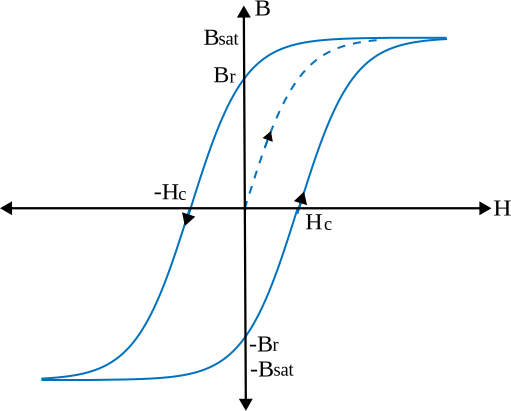
\includegraphics[width=0.475\textwidth]{mag_curve.pdf}}&
			\subcaptionbox{}{\includegraphics[width=0.5\textwidth]{0450015_ind.pdf}}
	\end{tabular}
	\caption{(a) Qualitative hysteresis loop for an arbitrary magnetic material. At the beginning the dashed line is followed. (b) Inductance vs. current behavior of the inductor 7440450015 from Würth Elektronik, taken from the datasheet.}
	\label{fig:magnetization}
\end{figure}

\subsubsection{Core Losses, Concept of Complex Relative Permeability and its Dispersion}
In addition to the dependence of $\mu_\mathrm{r}$ on the amplitude of the applied signal, another phenomenon that must be considered when working with magnetic core inductors is the frequency dependence of the relative permeability (dispersion) and losses. To model this, the relative permeability can defined as a complex number
\begin{equation}\label{eqn:complex_mu1}
	\underline{\mu_\mathrm{r}} = \mu_re^{-j\delta_\mathrm{\mu}} = \mu_\mathrm{r}\cos(\delta_\mu) - j\mu_\mathrm{r}\sin(\delta_\mu) =: \mu_\mathrm{r}' - j\mu_\mathrm{r}''\,.
\end{equation}
Here $\underline{\mu_\mathrm{r}}$ is the complex relative permeability, $\mu_\mathrm{r}$ is the relative permeability, $\delta_\mu$ is the loss angle of the magnetic material ($\tan(\delta_\mu)$: loss factor), $\mu_\mathrm{r}'$ and $\mu_\mathrm{r}''$ are the real and imaginary parts of the complex relative permeability and all these quantities are frequency dependent. For practical cores, $\delta_\mu \ll 1$, so using $\cos(\delta_\mu) \approx 1$ and $\sin(\delta_\mu) \approx \tan(\delta_\mu) \approx \delta_\mu$, \eqref{eqn:complex_mu1} can be simplified into 
\begin{equation} \label{eqn:complex_mu2}
	\underline{\mu_\mathrm{r}} = \mu_\mathrm{r} - j\mu_\mathrm{r}\tan(\delta_\mu) \quad\Longrightarrow\quad \mu_\mathrm{r}' = \mu_\mathrm{r} 
	\quad\mathrm{and}\quad
	\mu_\mathrm{r}'' = \mu_\mathrm{r}\tan(\delta_\mu)\,, 
\end{equation}
whereas $\mu_\mathrm{r}'$ relates to the relative permeability of the core, while $\mu_\mathrm{r}''$ relates to the amount of losses in the core. The losses in a magnetic core that are modeled with $\mu_\mathrm{r}''$ can be hysteresis losses, eddy current losses and the residual losses~\cite{snelling}. The hysteresis losses are described by the hysteresis loop in Fig.~\ref{fig:magnetization}. It arises because the magnetic flux density inside the core does not follow the externally applied AC input signal, but lags behind it~\cite{snelling}. The eddy current losses arise because the changing magnetic field induces loops of electric currents inside the material, which in turn cause resistive losses due to heat dissipation~\cite{snelling}. Nevertheless, for high resistivity magnetic cores such as ferrites, the eddy currents are weak at macroscopic level, so the eddy current losses can be neglected in them~\cite{wijn}.

\begin{figure}[ptb]
	\centering
	\includegraphics[width=0.475\textwidth]{fair_rite.pdf}
	\caption{Frequency response of the complex relative permeability for the 15~Material NiZn ferrite from Fair-Rite.}
	\label{fig:dispersion}
\end{figure} 
The frequency response of $\mu_\mathrm{r}'(\omega)$ and $\mu_\mathrm{r}''(\omega)$ of ferrite cores used in practice shows a behavior similar to a relaxation mechanism combined with a resonance behavior~\cite{wijn}. As an example, Fig.~\ref{fig:dispersion} shows the dispersion of the complex relative permeability of the 15~Material NiZn ferrite from Fair-Rite. In~\cite{wijn} it is explained that the dispersion of the domain wall motion and the spin rotation are the main contributors to the observed frequency dependence of the relative permeability. In~\cite{tsutaoka}, the author characterized the dispersion of relative permeability of polycrystalline ferrites as the superposition of the resonance of the domain wall motion and the resonance of the spin rotation, because in practical ferrites, the weighting of these two contributions to the total magnetization hence to the relative permeability can be very different~\cite{nakamura}. Therefore, both contributions must be taken into account. As a side note, polycrystalline ferrites are the most common type of ferrites and they are the ones discussed in this work. Their crystal microstructure consists of several grains in contrast to single grain (monocrystalline) ferrites~\cite{wijn}. For the frequency dependence of the complex relative permeability of polycrystalline ferrites, the author in~\cite{tsutaoka} came up with the following equation:
\begin{equation} \label{eqn:disp1}
	\underline{\mu_\mathrm{r}}(\omega) = 1 + \underline{\chi_\mathrm{sp}}(\omega)  +  \underline{\chi_\mathrm{dw}}(\omega)\,,
\end{equation}
where $\underline{\chi_\mathrm{sp}}$ is the contribution of the spin rotation to the magnetic susceptibility and $\underline{\chi_\mathrm{dw}}$ is the contribution of the domain wall motion to the magnetic susceptibility. For $\underline{\chi_\mathrm{sp}}$, the author uses the dispersion relation for spin rotation derived by Landau and Lipschitz in~\cite{landau} and for $\underline{\chi_\mathrm{dw}}$, he models the domain wall motion as a damped harmonic oscillator and uses the Lorentz's oscillator model~\cite{werkstoffe} and arrives at the following equation:
\begin{equation} \label{eqn:disp2}
	\underline{\mu_\mathrm{r}}(\omega) = 1 + \frac{(\omega_\mathrm{sp}+j\omega\alpha)\omega_\mathrm{sp}\chi_\mathrm{sp}^0}{(\omega_\mathrm{sp}+j\omega\alpha)^2-\omega^2} +  \frac{\omega_\mathrm{dw}^2\chi_\mathrm{dw}^0}{\omega_\mathrm{dw}^2-\omega^2+j\omega\beta}\,,
\end{equation}
where $\chi_\mathrm{sp}^0$ and $\chi_\mathrm{dw}^0$ are the contributions of spin rotation and domain wall motion to the magnetic susceptibility at low frequencies ($\omega \rightarrow 0$), $\omega_\mathrm{sp}$ and $\omega_\mathrm{dw}$ are the resonance frequencies of spin rotation and domain wall motion, respectively, and $\alpha$ and $\beta$ are damping factors~\cite{tsutaoka}. In Equations (3), (4) in~\cite{tsutaoka}, \eqref{eqn:disp2} is also separated into its real and imaginary parts, which is not repeated here. For large $\alpha$, the second term in \eqref{eqn:disp2} becomes the Debye relaxation equation~\cite{aee423}, hence the complex relative permeability becomes:
\begin{equation} \label{eqn:disp3}
	\underline{\mu_\mathrm{r}}(\omega) = 1 + \frac{\chi_\mathrm{sp}^0}{1+j\omega\tau} + \frac{\omega_\mathrm{dw}^2\chi_\mathrm{dw}^0}{\omega_\mathrm{dw}^2-\omega^2+j\omega\beta}\,,
\end{equation}
where $\tau$ is the relaxation time constant~\cite{wijn, aee423}. As an example, when trying to fit the frequency response in Fig.~\ref{fig:dispersion} with the above model, one obtains the curves shown in Fig.~\ref{fig:dispersion2} after applying a particle swarm optimization in MATLAB. From Fig~\ref{fig:dispersion2}(a), it can be seen that \eqref{eqn:disp2} models $\mu_\mathrm{r}'$ close to the measured data, except for the spike that is observed at \SI{1}{\mega\hertz}, which also seems to be the case in~\cite{nakamura, tsutaoka, aee423}. This also true for $\mu_\mathrm{r}''$ in Fig~\ref{fig:dispersion2}(b). There, it can be seen that the model is very close to the measured data at high frequencies. However, there is a moderate deviation at about \SI{1}{\mega\hertz} and at low frequencies. The deviation at \SI{1}{\mega\hertz} can be explained with the deviation of $\mu_\mathrm{r}'$ of the complex relative permeability. Because the real and imaginary parts of complex relative permeability are not independent from each other, but they follow the Kramers-Kronig relations~\cite{wijn}. Kramers-Kronig relations are simply mathematical relations that relate the real and imaginary parts of a complex function that is holomorphic in the upper half-plane of the complex plane, which is the case for the complex relative permeability~\cite{kramers}.
\begin{figure}[ptb]
	\centering
	\begin{tabular}{cc}
		\subcaptionbox{}{\includegraphics[width=0.5\textwidth]{fit1.pdf}}&
		\subcaptionbox{}{\includegraphics[width=0.5\textwidth]{fit2.pdf}}
	\end{tabular}
	\caption{(a) Real part and (b) imaginary parts of the complex relative permeability of Fair-Rite 15~Material in Fig.~\ref{fig:dispersion} is fitted with \eqref{eqn:disp2}. Following parameters are obtained from the particle swarm optimizer in MATLAB: $\chi_\mathrm{sp}^0 = 1433$, $\omega_\mathrm{sp} = \SI[per-mode=symbol]{9e9}{\radian\per\second}$, $\alpha = 427.7 $; $\chi_\mathrm{dw}^0 = 147$, $\omega_\mathrm{dw} = \SI[per-mode=symbol]{1.1e9}{\radian\per\second}$, $\beta = \SI[per-mode=symbol]{8.3e9}{\radian\per\second}$}
	\label{fig:dispersion2}
\end{figure}

Finally, for air core inductors in SMT, temperature dependence, saturation, dispersion, and the losses of the magnetic core are obviously absent. Therefore, they have much better linearity, quality factors and manufacturing tolerances. The disadvantage, however, is that their inductance is quite limited. It is at most in the order of \SI{100}{\nano\henry}.

\subsection{Equivalent Circuit}
In an electrical circuit, modeling a physical inductor as an ideal inductor $L$ is not accurate, especially at high frequencies. This is because additional physical effects that a physical inductor is subject to and that are not modeled by the ideal inductor can drastically change the components behavior. In the electrical circuit model of the physical inductor, these effects are taken into account by connecting parasitic components to the ideal inductor. Fig.~\ref{fig:Leqv} shows the equivalent circuit of an inductor, that can more accurately model the behavior of the physical inductor. In this circuit, the series resistance $R_\mathrm{S}$ models the real power losses due to the DC resistance of the wire, which can be significant for inductors using thin wires with many turns. Ideally this resistance is zero. Besides, at higher frequencies, additional resistance occurs due to the skin-effect and proximity effect, which can be included as the frequency-dependent part of $R_{\mathrm{S}}$. In this work, $R_{\mathrm{S}}$ corresponds only to the DC resistance of the component. The parallel resistance $R_{\mathrm{P}}$ models the real power losses due to the losses in the magnetic core, as described in the previous section. Ideally the parallel resistance is infinite. The parallel capacitance in the equivalent circuit, which is ideally zero, is of great importance for modeling the high-frequency behavior of the inductor. There are three main physical effects that contribute to the parallel capacitance. The first is the capacitive coupling between the windings of the coil, the second is the capacitive coupling between the coil and the shield of the inductor, and the third is the capacitive coupling between the coil and the magnetic core~\cite{6732932}. In this work, the inductors are unshielded and the core is a NiZn ferrite core, which, as mentioned earlier, usually has a high resistance. Therefore, the contribution of the latter two can be neglected. The parallel capacitance $C_\mathrm{P}$ models the capacitive coupling between the neighboring windings of the physical inductor. From Fig.~\ref{fig:Leqv}, it can be seen that $L$ and $C_{\mathrm{P}}$ together form a parallel LC resonator. At low frequencies the LC resonator behaves more like an inductor. However, this is no longer the case after the resonance frequency, which is given by
\begin{equation}\label{eqn:fSRL} \
	f_{\mathrm{SR}} = \frac{1}{2\pi\sqrt{LC_\mathrm{P}}}\,.
\end{equation}
This frequency is called the self-resonance frequency of the inductor and above this frequency the physical inductor  behaves more like a capacitor. At resonance the parallel LC resonator has infinite impedance, so the impedance of the inductor at the self-resonance frequency is determined by the parallel resistance $R_{\mathrm{P}}$.
\begin{figure}[ptb]
	\centering
	\includegraphics[width=0.5\textwidth]{inductor_eqv.pdf}
	\caption{Equivalent circuit diagram of an inductor in Spice simulators.}
	\label{fig:Leqv}
\end{figure}

\subsection{Design Equations for Single Layer Air Core Inductors}
\begin{figure}[ptb]
	\centering
	\includegraphics[width=0.4\textwidth]{singlelayer.pdf}
	\caption{Geometry parameters of a single layer air core inductor.}
	\label{fig:air_core}
\end{figure}
This section presents the design equations that can be used for predicting the geometry parameters as well as for calculating the values of the parasitic components of single layer air core inductors. These values ​​of the parasitic components will be used to compare with the data released by the manufacturer to verify the predicted geometry. For single layer air core inductors illustrated in Fig.~\ref{fig:air_core}, following geometry parameters are defined: $N$ is the number of turns, $l$ is the center-to-center length of the coil, $d$ is the center-to-center diameter, $d_\mathrm{i}$ is the wire diameter, $\delta$ is the insulation thickness and $d_\mathrm{o} = d_\mathrm{i}+2\delta$ is the wire diameter including the insulator. The inductance of such coil can be precisely calculated using the following equations~\cite{nagaoka}:
\begin{equation}\label{eqn:aircoil1}
	L_\mathrm{s} = N^2\mu_0\frac{\pi (d/2)^2}{l}k\,,
\end{equation}
where $k$ is the Nagaoka correction factor that is calculated using
\begin{equation}
	k = \frac{4}{3\pi}\frac{1}{\kappa'}\left(\frac{\kappa'^2}{\kappa^2}(K(\kappa)-E(\kappa))+E(\kappa)-\kappa\right)\,
	\quad \text{with} \quad
	\kappa = \frac{d}{d^2+l^2}
	\quad \text{and} \quad
	\kappa' = \frac{l}{d^2+l^2}\,,
\end{equation}
whereas $K(\cdot)$ and $E(\cdot)$ are the complete elliptic integrals of the first and second kind respectively~\cite{nagaoka}. Notice the subscript $s$ (stands for "sheet") on the inductance symbol. These equations are derived by assuming the coil windings to be infinitely thin current sheets~\cite{rosa}. In reality, the wires have a finite dimension. To make the result even more precise, Rosa's formula for round wire correction can be applied and the total inductance of the coil can be calculated using
\begin{equation}\label{eqn:aircoil2}
	L = L_\mathrm{s} - \mu_0\frac{d}{2}N(k_\mathrm{s}+k_\mathrm{m})\,,
\end{equation}
where $k_\mathrm{s}$ is the self-inductance correction factor and $k_\mathrm{m}$ is the mutual inductance correction factor~\cite{rosa}. The factors $k_\mathrm{s}$ and  $k_\mathrm{m}$ can be read from Tables VII and VIII in~\cite{rosa}, respectively. For checking the feasibility of the predicted geometry the DC resistance of the coil can be calculated using 
\begin{equation} \label{eqn:aircoil3}
	R_\mathrm{S} = \rho_\mathrm{c}\frac{l_\mathrm{w}}{\pi (d_\mathrm{i}/2)^2}\,
	\quad \text{with wire length} \quad 
	l_\mathrm{w} = N\sqrt{(\pi d)^2+(l/N)^2}\,,
\end{equation}
where $\rho_\mathrm{c}$ is the specific resistance of copper and equals \SI{1.72e-8}{\ohm\meter}. The latter equation is simply the length of a helix. Moreover, the parasitic capacitance of a single layer inductor can be approximated using Medhurst's empirical equation in~\cite{medhurst} 
\begin{equation} \label{eqn:aircoil4}
	C_\mathrm{P} = \frac{4\varepsilon_0l}{\pi}\left(1+0.71\frac{d}{l}+2.4\left(\frac{d}{l}\right)\strut^{1.5}\right)\,,
\end{equation}
where $\varepsilon_0$ is the vacuum permittivity.
\subsection{Design Equations for Multilayer Air Core Inductors}
\begin{figure}[ptb]
	\centering
	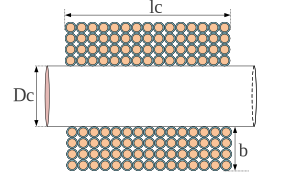
\includegraphics[width=0.475\textwidth]{multilayer.pdf}
	\caption{Geometry parameters of a multilayer coil.}
	\label{fig:multilayer}
\end{figure} 
The drum core inductors modeled in this work consist of multilayer coils that are wound in a square shape around a ferrite core. However, despite the ferrite core, the design equations for multilayer air core inductors are still needed for predicting the geometry of the coil. In this work, the geometry of a multilayer coil is mathematically modeled in a similar way as in~\cite{6732932}, however the coil in that work is circular shaped, whereas in this work the coil is square shaped. Fig.~\ref{fig:multilayer} shows the geometry for a square shaped multilayer coil which is cut in its mid-plane. Following geometry parameters are defined for it: $N$ is the total number of windings, $N_\mathrm{V}$ is the number of windings in one layer, $N_\mathrm{L}$ is the number of layers, $d$ is the side length of the rod, which is assumed to be filled with air for now, $d_\mathrm{i}$ is the inner diameter of the wire, $d_\mathrm{o}$, is the outer diameter of the wire, $\delta$ is the insulator thickness, $l$ is the total length of the coil, $\xi_z$ is the gap distance between two adjacent turns in the same layer and $\xi_r$ is the negative of the vertical distance between two turns in adjacent layers~\cite{6732932}. The parameter $\xi_r$ is helpful for including the hexagonally wound multilayer coils in the model, which means that one winding in the upper layers is located between two windings in the lower layer~\cite{6732932}. However in this work the coil is assumed to be wound orthogonally, which means that the windings in the upper and lower layers are perfectly aligned on the $z$-axis, which corresponds to the shape shown in Fig~\ref{fig:multilayer}~\cite{6732932}. For orthogonal windings, $\xi_r = 0$ holds. Furthermore, $r_j$ is the distance of the center point of $j$-th winding from the $z$-axis and $z_j$ is the distance of the center point of $j$-th winding from the $r$-axis. The inductance of a multilayer air core coil can be calculated using 
\begin{equation} \label{eqn:multilayer_eqn1}
	L_\mathrm{air} = \sum_{j=0}^{N}L_j + \sum_{j=0}^{N}\sum_{\substack{k=0 \\ k\neq j}}^{N} M_{jk}\,,
\end{equation}
whereas $L_j$ is the self-inductance of the $j$-th winding and $M_{jk}$ is the mutual inductance between the $j$-th and $k$-th windings. The self-inductance of a square winding (square shaped loop) can be calculated using Equation (60) in~\cite{grover2013}. After converting the equation from CGS units into SI units one obtains
\begin{equation}  \label{eqn:multilayer_eqn2}
	L_j = \mu_0\frac{2r_j}{\pi}\left(\ln\left(\frac{2r_j}{(d_i/2)}\right) - 0.77401\right)\,.
\end{equation}
The mutual inductance between two square loops can be approximated by the mutual inductance of two square current sheets and can be calculated using Equation (11) in~\cite{cheng}
\begin{equation} \label{eqn:multilayer_eqn3}
	\begin{aligned}
		M = \frac{2\mu_0}{\pi}\Bigg[&
		\sqrt{2(a+c)^2+z^2}+\sqrt{2(a-c)^2+z^2}-2\sqrt{2a^2+2c^2+z^2} \\ &-(a+c)\arctanh{\left(\frac{a+c}{\sqrt{2(a+c)^2+z^2}}\right)}-(a-c)\arctanh{\left(\frac{a-c}{\sqrt{2(a-c)^2+z^2}}\right)} \\
		&+(a+c)\arctanh{\left(\frac{a+c}{\sqrt{2a^2+2c^2+z^2}}\right)}+(a-c)\arctanh{\left(\frac{a-c}{2a^2+2c^2+z^2}\right)}\Bigg]\,,
	\end{aligned}
\end{equation}
where $2a$ is the side length of the first sheet and $2c$ is the side length of the second sheet and $z$ is the distance apart. To make \eqref{eqn:multilayer_eqn3} compatible with the model used in this work and thus to obtain $M_{jk}$ in \eqref{eqn:multilayer_eqn1}, $a$ needs to be replaced with $r_j$, $c$ needs to be replaced with $r_k$, and $z$ needs to be replaced with $\abs{z_j - z_k}$. In addition, a round wire correction can be applied to \eqref{eqn:multilayer_eqn3} by using the method described in Section II-C of~\cite{cheng} and using Equation (13) in~\cite{cheng}. Moreover the DC resistance of a multilayer coil can be calculated with
\begin{equation} \label{eqn:multilayer_eqn4}
	R_\mathrm{S} = \rho_\mathrm{c}\frac{l_\mathrm{w}}{\pi(d_\mathrm{i}/2)^2}\,, 
\end{equation}
where $l_\mathrm{w}$ is the wire length, which can be calculated with
\begin{equation} \label{eqn:multilayer_eqn5}
	l_\mathrm{w} = \sum_{j=0}^{N}\left(4\sqrt{(2r_j)^2+(p/4)^2}\right)\,,
\end{equation}
where $p = d_\mathrm{o}+\xi_z$ is the pitch of the windings. Unfortunately, analytical equations are not available for calculating the parasitic capacitance of a square-shaped multilayer coil. In~\cite{6732932}, analytical equations for circular shaped multilayer coils were derived. However, after testing the equation with CST simulations, it turns out that it cannot be applied to square-shaped coils. Therefore, the parasitic capacitance $C_\mathrm{P}$ is not used to check the feasibility of the predicted geometry.

\subsection{3D Modeling of SMD Inductors}
After introducing the relevant theory, the inductors can be modeled. The inductors that are modeled in this work are the \SI{100}{\nano\henry} air core inductor 744912210, \SI{1.5}{\micro\henry} unshielded drum core inductor 7440450015, \SI{2.2}{\micro\henry} unshielded drum core inductor 744045002, all manufactured by Würth Elektronik. The only information that can be found about these inductors is their datasheet and their Spice model, which contains the parasitic component values for the equivalent circuit shown in Fig.~\ref{fig:Leqv}. However, the manufacturer shares the picture and the CAD model for other inductors in the corresponding inductor family, which are used as a reference for the inductor models in this work.

\subsubsection{Modeling of 744912210 Air Core Inductor by Würth Elektronik}
The first inductor to be modeled is a \SI{100}{\nano\henry} air core inductor with the model number 744912210. A quick look at the CAD model for the \SI{120}{\nano\henry} 744912212 inductor, shared by the manufacturer, shows the wire diameter to be \SI{0.38}{\milli\meter}, so 26 or 27 gauge wire is assumed, which corresponds to $d_\mathrm{i} = \SI{0.36}{\milli\meter}$ or $d_\mathrm{i} = \SI{0.4}{\milli\meter}$, respectively. In both cases, for standard enameled magnet wire, $\delta = \SI{0.0185}{\milli\meter}$~\cite{electronbunker}. From the datasheet of the component, $l = \SI{4.32}{\milli\meter} \pm \SI{0.39}{\milli\meter}$ and $d = \SI{2.9}{\milli\meter} \pm \SI{0.78}{\milli\meter}$ can be read. In the next step, a MATLAB script is created that implements the equations introduced in the previous sections. The geometry of the inductor is predicted using \eqref{eqn:aircoil1}~-~\eqref{eqn:aircoil2} and its feasibility is checked using \eqref{eqn:aircoil3}, \eqref{eqn:aircoil4} and the obtained values are compared to the values shared by the manufacturer for the equivalent circuit in Fig,~\ref{fig:Leqv}. By experimenting with different geometry parameters in their specified interval, some valid coil geometries are obtained, which are summarized in Table~\ref{tab:valid_geom}.
\begin{table}[ptbh]
	\centering
	\begin{tabular}{|c| c c c c c|}
		\hline
		Coil Number & $N$ & $d$ (\SI{}{\milli\meter}) & $l$ (\SI{}{\milli\meter}) & $d_\mathrm{i}$ (\SI{}{\milli\meter}) & $\delta$ (\SI{}{\milli\meter})\\
		\hline
		$\#1$ & 8 & 3.2  & 4.32 & 0.4 & 0.0185 \\
		$\#2$ & 9 & 2.9 & 4.32 &  0.4 & 0.0185\\
		$\#3$ & 10 & 2.6 & 4.5 & 0.4 & 0.0185\\
		\hline
	\end{tabular} 
	\caption{Valid geometries from the analytical equations for the air core inductor 744921210.}
	\label{tab:valid_geom}
\end{table}
Next, each coil geometry is implemented in CST and the parasitic component values from CST simulations are compared to the data from the manufacturer. The DC resistance $R_\mathrm{S}$ is obtained from the low-frequency, full-wave frequency domain solver at \SI{1}{\hertz}. Except for disabling the adaptive mesh refinement, all other settings in the "Transformers, Chokes" template are left at default. The inductance $L$ and the self-resonance frequency of the component are obtained from the high-frequency, frequency domain solver in CST and the default simulation settings from the template "EMC - Common Mode Chokes" are kept. The inductance is read at \SI{150}{\mega\hertz}, in accordance with the datasheet. Subsequently, the coil geometry with the simulation results closest to the data shared by the manufacturer is selected. This correspond to the coil \#3 in the Table~\ref{tab:valid_geom} and the 3D model of the component is shown in Fig.~\ref{fig:744912210}. Table~\ref{tab:air_core_results} summarizes the important results from the analytical equations, from CST and compares them to the values provided by the manufacturer. The parallel capacitance in CST simulations is calculated from the self-resonance frequency using \eqref{eqn:fSRL}.
\begin{table}[ptbh]
	\centering
	\begin{tabular}{|c|c| c c c c|}
		\hline
		Model number& Results from & $L\,(\SI{}{\nano\henry})$ & $R_\mathrm{S}\,(\SI{}{\milli\ohm})$ & $C_\mathrm{P}\,(\SI{}{\pico\farad})$ & $f_\mathrm{SR}\,(\SI{}{\giga\hertz})$\\
		\hline
		&Equations & 105 & 12.1 & 0.125& 1.390\\
		744912210 & CST & 100 & 12.8 &  0.131 & 1.389\\
		&Datasheet & $100\pm5\%$ & $< 12.3$ & $< 0.176$ & $> 1.2$\\
		\hline
	\end{tabular} 
	\caption{Important values obtained from analytical equations and from CST are compared with the data provided by the manufacturer for the air core inductor 744912210.}
	\label{tab:air_core_results}
\end{table}
\begin{figure}
	\centering
	\includegraphics[width=0.4\textwidth]{744912210.png}
	\caption{3D model of the inductor 744912210 in CST.}
	\label{fig:744912210}
\end{figure}

\subsubsection{Modeling 7440450015 and 744045002 Drum Core Inductors by Würth Elektronik}
The inductors 7440450015 and 744045002 belong to the WE-LQ SMT inductor family from Würth Elektronik. The manufacturer shares the 3D CAD model of the \SI{1}{\micro\henry} inductor in the family, 744045001, shown in Fig.~\ref{fig:744045001}. Since the inductors implemented in this work are very similar to 744045001, they are created based on it.
\begin{figure}[ptb]
	\centering
	\includegraphics[width=0.5\textwidth]{744045001.png}
	\caption{CAD model of the inductor 744045001. The inductors 7440450015 and 744045002 are based on this model.}
	\label{fig:744045001}
\end{figure}
A quick inspection of the CAD model shows that the component is a multilayer inductor created by winding a 33-34 gauge copper wire around a NiZn ferrite rod with a square cross-section in multiple layers. For now the relative permeability of the ferrite core is ignored because it is impossible to predict it, as different NiZn ferrites can have different relative permeabilities depending on the chemical composition as well as the microstructure such as grain sizes and porosity~\cite{wijn}. The square cross-section of the rod has dimensions $\SI{1.4}{\milli\meter}\times\SI{1.4}{\milli\meter}$ and its length is $\SI{1.3}{\milli\meter}\pm\SI{0.3}{\milli\meter}$. The fundamental geometry parameters that needs to be predicted are \{$N$, $d_\mathrm{i}$, $\delta$, $l$, $\xi_z$, $\xi_r$\}. In this work, the parameters $\xi_z$ and $\xi_r$ are set to \SI{0.005}{\milli\meter}. This is the offset value that is used when modeling the coils in CST, so that the wires do not overlap, which can lead to mesh errors. The total length of the coil $l$ is assumed to be $\SI{1}{\milli\meter} - \SI{1.2}{\milli\meter}$, close to the rod length. Based on the CAD model, the wire diameter is predicted to be 33 or 34 gauge, so a 34 gauge wire ($d_i = \SI{0.16}{\milli\meter}$) is chosen in the first step. For standard 33 and 34 gauge enameled magnet wire, the insulation thickness is $\delta = \SI{0.01}{\milli\meter}$~\cite{electronbunker}. Consequently, the number of unknowns are reduced to one. For the prediction of $N$ the inductance of the coil needs to be calculated using \eqref{eqn:multilayer_eqn1}~-~\eqref{eqn:multilayer_eqn3}. However to be able to use \eqref{eqn:multilayer_eqn1}~-~\eqref{eqn:multilayer_eqn3}, one must know the inductance of the coil without the ferrite core, $L_\mathrm{air}$. This value can be taken from the inductance vs. current graph in the component's datasheet. As explained earlier, at higher currents the coil enters magnetic saturation and its relative permeability drops to unity. Therefore, the coil effectively becomes an air core coil. The inductance vs. current relationship is already shown for 7440450015 in Fig.~\ref{fig:magnetization}(b). From this graph $L_{\mathrm{air}}$ can be read as approximately \SI{0.23}{\micro\henry}, also $\mu_{\mathrm{r,eff}} = L_{\mathrm{f}}/L_{\mathrm{air}} = 6.52$. As a numerical example, using \eqref{eqn:demag}, the demagnetizing factor $D$ of the core can be calculated as 0.11. When considering the core in Fig~\ref{fig:744045001} without the top and bottom parts and only the rod in the middle with the dimensions $\SI{1.4}{\milli\meter}\times\SI{1.4}{\milli\meter}\times\SI{1.3}{\milli\meter}$, the demagnetization factor becomes approximately 0.3631, which can be read from Table I in~\cite{moskowitz}. This means the top and bottom parts of the core achieves a 3-4 times gain in the demagnetization factor. In the next step, a MATLAB script is implemented that uses \eqref{eqn:multilayer_eqn1}~-~\eqref{eqn:multilayer_eqn3}, as well as the round wire correction method described in~\cite{cheng}. With the goal $L_\mathrm{air} = \SI{0.23}{\micro\henry}$, the equations give $N = 12$ and the exact coil length $l$ becomes \SI{1.08}{\milli\meter}, thus considering the geometry parameters in Fig.~\ref{fig:multilayer}, $N_\mathrm{V} = 6$, and $N_\mathrm{L} = 2$ are obtained. Using \eqref{eqn:multilayer_eqn4} and \eqref{eqn:multilayer_eqn5}, for the predicted geometry of 7440450015, $R_\mathrm{S} = \SI{0.073}{\ohm}$ is obtained. Applying the same steps for 744045002, using a 33 gauge wire and targeting  $L_\mathrm{air} = \SI{0.32}{\micro\henry}$, $N = 15$, $N_\mathrm{V} = 5$, $N_\mathrm{L} = 3$ and $l = \SI{1}{\milli\meter}$ are obtained. Moreover for the predicted geometry of 744045002, $R_\mathrm{S} = \SI{0.082}{\ohm}$, is obtained. 

The inductors are then built in CST and Fig.~\ref{fig:3d_models} shows a picture of them. Unlike the CAD model from Würth Elektronik, the models in this work also include polyimide insulators with the relative permittivity $\varepsilon_\mathrm{r} = 3.5$ around the copper wires. In the next step, both coils are simulated using the low-frequency, full-wave frequency domain solver in CST. Again, except for disabling the adaptive mesh refinement, all other settings in the "Transformers, Chokes" template are left at default. The inductors are simulated at \SI{1}{\hertz}, \SI{1}{\kilo\hertz}, and \SI{1}{\mega\hertz} frequencies. The supply voltage is \SI{100}{\milli\volt}, the DC resistance is read at \SI{1}{\hertz}, and the inductance is read at \SI{1}{\mega\hertz}, all in accordance with the test conditions in the datasheets. Besides, the unknown parameter $\mu_\mathrm{r}$ of the ferrite cores is set to one. For 7440450015 the simulation results show $L_\mathrm{air} = \SI{0.216}{\micro\henry}$, $R_\mathrm{S} = \SI{0.077}{\ohm}$, and for 744045002 $L_\mathrm{air} = \SI{0.333}{\micro\henry}$, $R_\mathrm{S} = \SI{0.086}{\ohm}$ which are close enough to the obtained values from the analytical equations. The relative permeability of the ferrite core can now be determined using a parameter sweep in CST. For this purpose the high-frequency, frequency domain solver is used and the default simulation settings from the template "EMC - Common Mode Chokes" are kept at default. The relative permeability is defined as a variable and swept from 0 to 50. The value that gives the required inductance, $L_\mathrm{f}$, is chosen. For 7440450015, $\mu_\mathrm{r} = 22$ and for 744045002, $\mu_\mathrm{r} = 25$ are obtained. These values ​​make sense because the resonance frequencies for spin rotation and domain wall motion are inversely proportional to the relative permeability according to Equations (29)--(32) in~\cite{wijn}. Since these inductors are designed to operate at RF frequencies, their relative permeability must be low as the relative permeability starts to decrease around the resonance frequency. 

For completeness the dispersion of the relative permeabilities are also included. It had to be modeled using 1st order Debye model, because CST does not have a feature to optimize the parameters of the combined dispersion model in \eqref{eqn:disp2}, defined in a VBA script. The equation of the Debye model corresponds to the second term in \eqref{eqn:disp3}: $\underline{\mu_\mathrm{r}}(\omega)= 1+(\omega_\mathrm{0}^2\chi^0)/(1+j\omega\tau)$, where $\tau$ is the relaxation time constant, and $\chi^0$ is the magnetic susceptibility at low frequencies. The parameter $\chi^0 = \mu_\mathrm{r}-1 = 21$ and the parameter $\tau$ of the model is determined with an optimization in CST, so that the parallel resistance at the self-resonance frequency (which corresponds to the parallel resistance in the equivalent circuit and is directly related to the core's losses) matches the value given by the manufacturer. At the end of the optimization for 7440140015 $\tau = \SI{0.95}{\nano\second}$ and for 744045002 $\tau = \SI{0.65}{\nano\second}$ are obtained. Moreover, the high frequency solver can be used to read the self-resonance frequency and hence the parasitic capacitance from \eqref{eqn:fSRL}. For 744045015 $f_\mathrm{SR} = \SI{145}{\mega\hertz}$, $C_\mathrm{P} = \SI{0.834}{\pico\farad}$ and for 744045002 $f_\mathrm{SR} = \SI{123}{\mega\hertz}$, $C_\mathrm{P} = \SI{0.72}{\pico\farad}$ are obtained. Table~\ref{tab:drum_core_result} summarizes the final form of all relevant parameters for 7440450015 and 744045002 in CST. In addition, Table~\ref{tab:calc_compare} shows the results of the analytical equations and the results of the CST simulations and compares them  with the data provided by the manufacturer. This includes both the datasheet and the Spice model. The difference between parasitic capacitances $C_\mathrm{P}$ thus self-resonance frequencies can be attributed to manufacturer using a different insulation material with eventually higher relative permittivity but also to the orientation of the windings in the real component. Because although the parameters $\xi_r$ and $\xi_z$ do not have a significant impact on the inductance, they still have a moderate impact on the capacitance of the windings~\cite{6732932}. Finally, Fig.~\ref{fig:cstvsmanuf_imp}(a) and Fig.~\ref{fig:cstvsmanuf_imp}(b) compares the $\abs{\underline{Z_\mathrm{L}}(\omega)}$ results from CST's high-frequency, frequency domain solver with the Spice model simulation results for 7440450015 and 744045002 respectively.
\begin{table}[ptbh]
	\centering
	\begin{tabular}{|c|c c c c c c c c c|}
		\hline
		Inductor & $L_\mathrm{f}\,(\SI{}{\micro\henry})$ & $L_{\mathrm{air}}\,(\SI{}{\micro\henry})$ & $\mu_\mathrm{r}$ & $\mu_\mathrm{r,eff}$ & D & $\tau\,(\SI{}{\nano\second})$ & $N$ & $N_\mathrm{L}$ & $N_\mathrm{V}$\\
		\hline
		 7440450015 & 1.50 & 0.216 & 22 & 6.94 & 0.11 & 0.95  & 12 & 2 & 6\\
		 744045002 & 2.23 & 0.333 & 25 & 6.67 & 0.11 & 0.65  & 15 & 3 & 5\\
		\hline
	\end{tabular}
	\begin{tabular}{|c| c c c c c c c|}
		\hline
		Inductor & $l\,(\SI{}{\milli\meter})$ & $d\,(\SI{}{\milli\meter})$ & $d_\mathrm{i}\,(\SI{}{\milli\meter})$ & $\delta\,(\SI{}{\milli\meter})$ & $d_\mathrm{o}\,(\SI{}{\milli\meter})$ & $\xi_z\,(\SI{}{\milli\meter})$ & $\xi_r\,(\SI{}{\milli\meter})$\\
		\hline
		7440450015 & 1.08 & 1.4 & 0.16 & 0.01 & 0.18 & 0.005 & -0.005 \\
		744045002 & 1.00 & 1.4 & 0.18 & 0.01 & 0.20 & 0.005  & -0.005 \\
		\hline
	\end{tabular}
	\caption{Geometry parameters as well as material parameters predicted for 7440450015 and 744045002.}
	\label{tab:drum_core_result}
\end{table}
\begin{figure}[ptb]
	\centering
	\begin{tabular}{cc}
		\subcaptionbox{}{\includegraphics[width=0.475\textwidth]{7440450015.png}}&
		\subcaptionbox{}{\includegraphics[width=0.475\textwidth]{744045002.png}}
	\end{tabular}
	\caption{3D models of the drum core inductors in CST. (a) 7440450015 and (b) 744045002.}
	\label{fig:3d_models}
\end{figure}
\begin{table}[ptbh]
	\centering
	\begin{tabular}{|c|c|c c c c c c|}
		\hline
		Model number & Results from & $L_\mathrm{f}\,(\SI{}{\micro\henry})$ & $L_\mathrm{air}\,(\SI{}{\micro\henry})$ & $R_\mathrm{S}\,(\SI{}{\ohm})$ & $R_\mathrm{P}\,(\SI{}{\ohm})$ & $C_\mathrm{P}\,(\SI{}{\pico\farad})$ & $f_\mathrm{SR}\,(\SI{}{\mega\hertz})$\\
		\hline
		  & Equations & -- & 0.229 & 0.073 & -- & -- & --\\
		 \multirow{ 2}{*}{7440450015} & CST & 1.5 & 0.216 & 0.077 & 3330.8 & 0.834 & 145\\
		  & LTSpice & 1.5 & -- & 0.072 & 3303.9 & 1.155 & 121\\
		  & Datasheet & $1.5\pm20\%$ & 0.235 & < 0.090 & -- & $\approx 1$ & $\approx 130$\\
		 \hline
		  & Equations & -- & 0.404  & 0.082 & -- & -- & --\\
		 \multirow{ 2}{*}{744045002} & CST & 2.23 & 0.333 & 0.086 & 8002.9 & 0.72 & 123\\
		  & LTSpice & 2.2 & --  & 0.088 & 7826.2 & 0.863 & 120\\
		  & Datasheet & $2.2\pm20\%$ & 0.32 & < 0.110 & -- & $\approx1.8$ & $\approx80$\\
		\hline
	\end{tabular} 
	\caption{Important results from analytical equations and from CST simulations are compared with the data provided by the manufacturer, taken from the datasheets and the Spice models.}
	\label{tab:calc_compare}
\end{table}
\begin{figure}[ptb]
	\centering
	\begin{tabular}{cc}
		\subcaptionbox{}{\includegraphics[width=0.475\textwidth]{cstvsmanuf_0015.pdf}}&
		\subcaptionbox{}{\includegraphics[width=0.475\textwidth]{cstvsmanuf_002.pdf}}
	\end{tabular}
	\caption{Comparison between the $\abs{\underline{Z_\mathrm{L}}(\omega)}$ values from CST and simulation of manufacturer's Spice model (a) for 7440450015 and (b) for 744045002.}
	\label{fig:cstvsmanuf_imp}
\end{figure}


\section{Capacitors}
In surface mount technology, ceramic capacitors, tantalum capacitors and polarized aluminum polymer capacitors are the most common types of capacitors~\cite{digikey}. Among ceramic capacitors, multilayer ceramic capacitors (MLCC) are the most widely used and popular~\cite{digikey}. 
\subsection{Theory of Multilayer Ceramic Capacitors}
\begin{figure}[ptb]
	\centering
	\includegraphics[width=0.5\textwidth]{mlcc.pdf}
	\caption{Inner structure of an MLCC.}
	\label{fig:mlcc}
\end{figure}
Fig.~\ref{fig:mlcc} shows the internal structure of an MLCC~\cite{5482787}. It consists of a stack of SMD-sized rectangular metal sheets on top of each other, with the gaps between the stacks filled with a dielectric made of ceramic material. The metal layers inside the MLCC form an interdigitated structure. By connecting two adjacent metal layers to different electrodes of the MLCC, a parallel connection is achieved between each capacitor pair, so that the total capacitance is the sum of the individual capacitances. The formula for the total capacitance of an MLCC can be given using the capacitance formula of a parallel plate capacitor as follows:
\begin{equation} \label{eqn:mlcc}
	C = N_{\mathrm{C}}\varepsilon_0\varepsilon_\mathrm{r}\frac{A}{d}\,,
\end{equation}
where $N_{\mathrm{C}}$ is the total number of metal layers, whereas in an MLCC there can be hundreds of metal layers~\cite{8094717}, $\varepsilon_0$ is the vacuum permittivity, $\varepsilon_\mathrm{r}$ is the relative permittivity of the dielectric, $A$ is the area where two adjacent metal layers are capacitively coupled to each other and $d$ is the distance between them~\cite{5482787}. Starting from \eqref{eqn:mlcc}, to increase the capacitance of an MLCC, the area of metal sheets can be increased, which increases the horizontal dimensions of the component. Also, the number of metal layers $N_{\mathrm{C}}$ could be increased which in turn increases the vertical dimension of the component. Another possibility would be bringing the metal layers closer to each other, thus decreasing $d$, which also allows increasing the number of metal layers for the same component dimensions. However, due to manufacturing constraints, there is a lower limit to the thickness of the ceramic material, which defines how thin it can be made~\cite{5482787}. Also, making the ceramic material thinner would weaken the insulation of the dielectric thus lowering the breakdown threshold of the electric field, so the capacitor's rated voltage would decrease. Another way to increase the capacitance would be to increase the relative permittivity $\varepsilon_{\mathrm{r}}$. In this respect, the ceramic capacitors are divided into classes. In class one, the dielectric is made of paraelectric substances such as titanium dioxide \ce{TiO2} and they can reach a relative permittivity of a few hundred~\cite{5482787}. Accordingly, the achievable capacitance is low, but they offer the highest linearity against changing voltages, temperatures and frequencies~\cite{5482787}. The class two ceramic capacitors use ferroelectric dielectrics such as barium titanat \ce{BaTiO3} and they can reach a much higher relative permittivity, up to ten thousand and more~\cite{5482787}. However, unlike class one, they have poorer linearity against temperature, voltage and frequency~\cite{5482787}. The frequency dependency comes from the dipole relaxation at higher frequencies, which can be described with the Debye relaxation model~\cite{werkstoffe}. There are also losses in the dielectric of the capacitor which are mainly the polarization losses. These losses can be modeled by introducing a complex relative permittivity in the same manner as in \eqref{eqn:complex_mu1} and \eqref{eqn:complex_mu2}.

\subsection{Equivalent Circuit}
\begin{figure}[ptb]
	\centering
	\includegraphics[width=0.5\textwidth]{capacitor_eqv.pdf}
	\caption{Equivalent circuit of a capacitor in Spice simulators.}
	\label{fig:cap_eqv}
\end{figure}
Fig.~\ref{fig:cap_eqv} shows the equivalent circuit of a capacitor. Additional parasitic components are added on top of the ideal capacitor $C$ to more accurately model the behavior of a physical capacitor. The series resistance $R_\mathrm{S}$ models the dielectric losses as well as the losses due to the finite resistance of the capacitor's connections. The skin-effect at higher frequencies can also be considered, but is not as severe as for the inductors. Ideally, this value should be zero. The parallel resistance $R_\mathrm{P}$ is the isolation resistance. It models the finite resistance of the dielectric and the leakage current caused by it. This value is ideally infinite. Finally, the series inductor models the inductance of the electrical connections of the capacitor, since every piece of conductor shows an inductive behavior to some extent. This inductance determines the high-frequency behavior of the component and is ideally zero. Similar to the equivalent circuit of the inductor, one can also observe an LC resonator here, but this time a series resonance circuit, for which the resonance frequency can be given same as \eqref{eqn:fSRL}, using the capacitance $C$ and the parasitic inductance $L_\mathrm{S}$ of the component. Below this frequency, the capacitor behaves similar to an ideal capacitor, but above this frequency it starts to behave more like an inductor. An LC resonator acts like a short circuit at the resonance frequency so the equivalent circuit becomes identical to the parallel connection of $R_{\mathrm{P}}$ and $R_{\mathrm{S}}$. Considering $R_{\mathrm{P}} \gg R_{\mathrm{S}}$, the circuit can be simplified to $R_{\mathrm{S}}$ at the resonance frequency. Compared to SMD inductors, SMD capacitors have much higher quality factors and better manufacturing tolerances. This can be easily seen by comparing the datasheets of some popular capacitors and inductors.

\subsection{3D Modeling of SMD Capacitors}
As explained previously, modeling an MLCC with its potentially hundreds of metal layers is not feasible due to the immense simulation times and hardware usage~\cite{8094717}. Instead, the brick modeling technique that is used by Modelithics and that is also recommended in~\cite{8094717} is followed. In that paper, the external geometry of the MLCC is modeled exactly. However, the internal geometry is modeled using a lumped element, containing manufacturer-released Spice model of the component. This simplification obviously introduces errors, but as long as the near-field measurements are made a few centimeters away from the board instead of  measuring directly around the components, the error should be negligible. First, the strongest electric fields are usually contained inside the component, the fields that exit from it are the fringing fields, and a few centimeters above the board these fringe fields become negligible. Second, the electric field generated by the traces of the board are generally more dominant than the fields of the component, so its contribution is not that significant. Both of these cases are confirmed by CST Simulations. Since the component contains the Spice model as a lumped component, it is not useful to show the simulation results, as they are identical to the simulations results in LTSpice. Fig.~\ref{fig:cst_mlcc} shows some of the 3D capacitor models implemented in CST. It can be seen that the external dimensions of the capacitors are exact but the interior contains a lumped component instead of a ceramic material and many metal layers.
\begin{figure}[ptb]
	\centering
	\begin{tabular}{cc}
		\includegraphics[width=0.4\textwidth]{885342008003.png}&
		\includegraphics[width=0.4\textwidth]{885012007087.png}
	\end{tabular}
	\caption{Two examples out of various capacitor models implemented in CST. (a) 885342008003, (b) 885012007087.}
	\label{fig:cst_mlcc}
\end{figure}
\section{Resistors}
Finally, SMD resistors, also called chip resistors, are introduced. The most common types of SMD resistors are thick/thin-film resistors~\cite{digikey}.
\subsection{Theory of SMD Resistors}
\begin{figure}[ptb]
	\centering
	\includegraphics[width=0.5\textwidth]{resistor.pdf}
	\caption{Inner structure of an SMD resistor.}
	\label{fig:smd_resistor}
\end{figure}
Fig.~\ref{fig:smd_resistor} shows the internal structure of an SMD resistor~\cite{vishay}. It has a fairly simple architecture. A resistive layer with the required total resistance is placed on a substrate. This layer is connected to the electrodes and protected from the outside by a protective film. The total resistance $R$ of the component can be given as follows
\begin{equation} \label{eqn:resistance_resistor}
	R = \rho\frac{l}{A}\,,
\end{equation}
where $\rho$ is the specific resistance of the resistive layer in \SI{}{\ohm\meter}, $l$ is the length of the resistive layer and $A$ is the area of its cross-section. The main non-idealities of an SMD resistor are the temperature dependence of its resistance and its thermal noise~\cite{vishay}. Besides, the resistors have a certain power rating, after which excessive heating happens and the component may be damaged. Also, the resistors have parasitic inductance and capacitance, which are tiny, but their impedance and admittance become significant at very high frequencies, generally at \SI{1}{\giga\hertz} and above. Apart from that, the SMD resistors are very reliable and robust components with good manufacturing tolerances.
\subsection{Equivalent Circuit}
\begin{figure}[ptb]
	\centering
	\begin{tabular}{cc}
		\subcaptionbox{}{\includegraphics[width=0.45\textwidth]{resistor_eqv1.pdf}}&
		\subcaptionbox{}{\includegraphics[width=0.45\textwidth]{resistor_eqv2.pdf}}
	\end{tabular}
	\caption{Equivalent circuits for SMD resistors. (a) For small resistances, (b) for large resistances.}
	\label{fig:Reqv}
\end{figure}
Fig.~\ref{fig:Reqv} shows two equivalent circuits for an SMD resistor. In addition to the ideal resistors, the series inductors are used to model the inductive behavior of the resistor terminals, and the parallel capacitors model the capacitance between the two electrodes on the opposite sides of the component. The first equivalent circuit in Fig.~\ref{fig:Reqv}(a) is used to model the resistors with low resistance, approximately up to \SI{100}{\ohm}. The impedance of this circuit shows an continuously increasing frequency response. The second circuit in Fig.~\ref{fig:Reqv}(b) is used for resistors with a resistance above approximately \SI{100}{\ohm}. The impedance of this circuit, on the other hand, shows a continuously decreasing frequency response.

\subsection{3D Modeling of SMD Resistors}
The SMD resistors modeled in this work are RCP1206W50R0GEB and RCP1206W100RGEB from Vishay Intertechnology. Based on the material and geometry information in the datasheet, a 3D structure similar to that shown in Fig.~\ref{fig:smd_resistor} is implemented. For simplicity, the outer, intermediate and internal electrodes are combined into a single electrode made of tin. Aluminum nitride is chosen as the substrate material and epoxy as the protective film in accordance with the the datasheet. Besides, the resistive layer is defined as a sheet resistance ($R_\mathrm{s} = \rho/t$, where t is the thickness of the resistive layer) in CST and its sheet resistance is determined using \eqref{eqn:resistance_resistor} such that the total resistance of the component equals the target resistance value. Modeling the resistive layer with the exact material type is not so practical because the exact resistance of the layer can be changed by controlling its chemical composition and the amount of the active material, in this case ruthenium oxide. Fig.~\ref{fig:cst_res}(a) shows the 3D model of the \SI{50}{\ohm} resistor RCP1206W50R0GEB in CST. Moreover, the frequency response of its impedance is shown in Fig.~\ref{fig:cst_res}(b). Notice the slight increase in the impedance in \SI{}{\giga\hertz} range. This behavior is expected, as explained in the previous section when explaining the equivalent circuits of SMD resistors.
\begin{figure}[ptbh]
	\centering
	\begin{tabular}{cc}
		\subcaptionbox{}{\includegraphics[width=0.45\textwidth]{RCP1206W50R0GEB.png}}&
		\subcaptionbox{}{\includegraphics[width=0.45\textwidth]{rcp.pdf}}
	\end{tabular}
	\caption{(a) 3D model of the \SI{50}{\ohm} resistor RCP1206W50R0GEB in CST. (b) Frequency behavior of its resistance.}
	\label{fig:cst_res}
\end{figure}

\chapter{Circuit Implementations} \label{chap:three}
In this work, the center frequencies of the implemented circuits are not important as long as they are in the low frequency range (in the order of $\SI{1}{\mega\hertz}$ in this work). Hence, the inductor models, which require most design effort, can be reused for all circuits, and the capacitance values of capacitors, can be adjusted to achieve the desired behavior of the circuit. This would cause center frequencies of the circuits to differ slightly from each other, but this is not the main concern of this work. Utilizing the components from the previous chapter, the circuits for testing the inverse source solver can be implemented. The implemented circuits include basic loop circuit, microstrip patch circuit, resistively terminated coplanar circuit well as basic resonant circuits using the previously designed SMD components such as bandpass filters, couplers and Wilkinson dividers, among which the filters and dividers are mentioned in this report. In this chapter, first, each type of circuit is briefly introduced, then the corresponding simulation results such as S-parameters and near-field simulation results are shown. Each circuit is implemented on a Rogers RO4003C board. The important parameters for Rogers RO4003C are summarized in Table~\ref{tab:subs_param}, where $h$ is the substrate height, $\tan(\delta)$ is the loss factor of the substrate, $d_\mathrm{Cu}$ is copper thickness, and $\sigma_\mathrm{Cu}$ is the specific conductivity of copper. The horizontal dimensions of the boards are different for different circuits. They are given in the corresponding sections. Furthermore, each circuit has only one input port and the input to them is through an SMA connector shown in Fig.~\ref{fig:sma}. The bottom two arms are connected to the bottom ground plane of the board and the top two arms are connected to the ground plane at the top metal layer. The center core of the connector is the input to the circuit. A discrete port from the center core to the outer conductor is defined as the input port for the simulations. By default, CST excites this port with \SI{1}{\watt} available power through a \SI{50}{\ohm} resistor at each frequency. For the near-field simulations the high-frequency, frequency domain solver is used and except setting the order of the solver to one, all other settings in the "EMC/EMI, Radiated Emission, Digital Signals, PCB" template are left at default.
\begin{table}
	\centering
	\begin{tabular}{|cccccc|}
		\hline
		$h$ & $\varepsilon_\mathrm{r}$ & $\tan(\delta)$ & Metallization & $d_\mathrm{Cu}$ & $\sigma_{Cu}$\\
		\hline
		\SI{1.524}{\milli\meter}&3.55 & 0.0027 & Copper & \SI{17.5}{\micro\meter} & \SI[per-mode=symbol]{5.8e7}{\siemens\per\meter}\\
		\hline
	\end{tabular} 
	\caption{Rogers RO4003C parameters.}
	\label{tab:subs_param}
\end{table}
\begin{figure}[htpb]
	\centering
	\begin{tabular}{cc}
		\includegraphics[width=0.4\textwidth]{SMA-1.png}
		\includegraphics[width=0.4\textwidth]{SMA-2.png}
	\end{tabular}
	\caption{SMA connector used for feeding the circuits.}
	\label{fig:sma}
\end{figure}
\begin{figure}[!bt]
	\centering
	\begin{tabular}{cc}
		\subcaptionbox{}{\includegraphics[width=0.5\textwidth]{loop.png}}
		\subcaptionbox{}{\includegraphics[width=0.45\textwidth]{csteqv1.pdf}}
	\end{tabular}
	\caption{(a) Implemented loop circuit in CST. (b) Low frequency equivalent circuit of the configuration in CST.}
	\label{fig:loop}
\end{figure}
\FloatBarrier
\section{Loop circuit}
The first circuit to examine is the loop circuit. Fig.~\ref{fig:loop}(a) shows the implemented loop circuit on a $\SI{50.8}{\milli\meter} \times \SI{50.8}{\milli\meter}$ board, whereas there is no ground plane at the bottom layer in order to avoid weakening of the created magnetic field due to eddy currents. The circuit a simple one turn conductor loop, broken at the bottom and fed through the SMA connector. The inner radius of the loop is \SI{17.5}{\milli\meter} and the wire width is \SI{3}{\milli\meter}. At low frequencies, the loop is simply a short circuit. Hence, the voltage drop across it is almost zero. For this reason, there exists almost no electric field over the loop. Nonetheless, current still flows through loop, creating a magnetic field. Therefore, in the near-field of this type of circuit, the magnetic field is dominant at low frequencies. The amount of current flowing through the loop is determined by the power setting and series resistance of the supply. By default, the available power of the source is \SI{1}{\watt}. This is the power one would measure on the load if the generator with \SI{50}{\ohm} series resistance is terminated with a \SI{50}{\ohm} load. The same power should also be on the \SI{50}{\ohm} resistor in series with the power source. Therefore, the source produces a total of \SI{2}{\watt} power. In addition, the loop is a short circuit at low frequencies. Therefore, Fig.~\ref{fig:loop}(b) becomes the equivalent circuit of this configuration. The total power of the source of \SI{2}{\watt} is thus dissipated only through the \SI{50}{\ohm} series resistor. The current can therefore be calculated using $P = 1/2Z\abs{\underline{I}}^2$ with $Z = \SI{50}{\ohm}$ and $P = \SI{2}{\watt}$, which gives a current magnitude of $\abs{\underline{I}} = \SI{0.282}{\ampere}$ through the loop at low frequencies, measured at the input port. At higher frequencies, this current decreases due to the voltage induced in the loop according to Lenz's law. Fig.~\ref{fig:loop_sim1}(a) shows the magnitude of the current through the loop. As calculated previously, the current through the loop at low frequencies is \SI{0.282}{\ampere}. At about \SI{410}{\mega\hertz} the current drops to zero. This is due to parallel resonance, since beside behaving as inductor, a loop wire also has some parasitic capacitance which causes a resonance at high frequencies. Moreover, Fig.~\ref{fig:loop_sim1}(b) shows the frequency dependence of the magnitude of the $S_{11}$-parameter. At low frequencies it is close to \SI{0}{\decibel}, because the voltage drop over the loop is zero and therefore its accepted power is also zero. Hence, the incident power wave $\underline{a_1}$ is totally reflected and it becomes the reflected power wave $\underline{b_1}$. From $\underline{S_{11}} = \underline{b_1}/\underline{a_1}$, $\abs{\underline{S_{11}}} = 1$ which equals \SI{0}{\decibel}. At very high frequencies, in the \SI{}{\giga\hertz} region, the loop behaves like an antenna. A loop antenna radiates approximately when its circumference equal one wavelength~\cite{balanis}. The circumference at the center of the wire is $2\pi\times\SI{19}{\milli\meter} = \SI{119}{\milli\meter}$. Therefore, from $f = c/\lambda$, the expected frequency at which the loop radiates, is around \SI{2500}{\mega\hertz}, which can also be seen in Fig.~\ref{fig:loop_sim1}, where the magnitude of the $S_{11}$-parameter drops below \SI{-10}{\decibel}.
\begin{figure}
	\centering
	\begin{tabular}{c}
		\subcaptionbox{}{\includegraphics[width=0.475\textwidth]{loop_cur.pdf}}\\
		\subcaptionbox{}{\includegraphics[width=0.475\textwidth]{loop_s11.pdf}}
	\end{tabular}
	\caption{(a) Magnitude of the current through the loop depending on the frequency. (b) Magnitude of the $S_{11}$-parameter depending on the frequency. Both measured at the input port.}
	\label{fig:loop_sim1}
\end{figure}
Furthermore, Fig.~\ref{fig:loop_sim2} shows the results of the near-field simulations. In these plots, the magnitude of the electric and magnetic field over the loop at different frequencies is shown on a $\SI{40}{\centi\meter} \times \SI{40}{\centi\meter}$ plane, \SI{3}{\centi\meter} above the circuit. The center point in the plots corresponds to the origin point in the sampling plane. In addition, the fields are displayed in logarithmic scale. The electric field is displayed between \SI{-20}{\dBVpm} and \SI{20}{\dBVpm}, while the magnetic field is displayed between \SI{-60}{\dBApm} and \SI{0}{\dBApm}. As expected, this circuit exhibits a typical low impedance behavior, where the magnetic field dominates and there is almost no electric field at low frequencies. As the frequency increases, the magnitude of the induced voltage increases, creating a stronger electric field across the loop. Relative to the scale used in Fig.~\ref{fig:loop_sim2}, one starts to recognize the electric field above \SI{10}{\mega\hertz}. Fig.~\ref{fig:loop_sim3} shows the average of the electric and magnetic field magnitudes in the sampling plane. From Fig.~\ref{fig:loop_sim3}(a) one can again see the weakness of the electric field at low frequencies and its build-up at higher frequencies. On the other hand, from Fig.~\ref{fig:loop_sim3}(b) one can see the dominance of the magnetic field at low frequencies. However, as the frequency increases the magnetic field first drops to low values before increasing again. This can be explained by the parallel resonance of the loop circuit at these frequencies, which causes the current to drop to zero as shown in Fig.~\ref{fig:loop_sim1}. However, according to Maxwell's equations, the source of magnetic fields can also be time-varying electric fields. Hence, despite almost zero current around the resonance point a weak magnetic field still exists due to the displacement current $j\omega\varepsilon\underline{\vec{E}}$. Moreover, the magnetic field and the electric field gradually increase at higher frequencies. This can again be explained by the fact that the time derivative terms in the Maxwell's equations become larger with increasing frequency and the magnetic and electric fields induce each other. Finally, Fig.~\ref{fig:loop_sim3}(c) shows the average wave impedance $Z_\mathrm{W} = \abs{\underline{\vec{E}}}/\abs{\underline{\vec{H}}}$ at different frequencies. It is computed by dividing the electric field and the magnetic field magnitudes on each point in the sampling plane and consequently by averaging the obtained values. Remember that the simulation results are collected planar, \SI{3}{\centi\meter} above the circuit. The boundary of the reactive near field is approximately at $\lambda/(2\pi)$~\cite{balanis}. So at low frequencies this value is high, which is why the sampling plane is in the near-field. In the near-field the measured fields are predominantly reactive fields, which means that the electric and magnetic field are out of phase and the imaginary part of the Poyting vector dominates~\cite{balanis}. These fields are stored around the circuit and do not radiate away~\cite{balanis}. In addition, the wave impedance in this region can differ greatly from the free-space wave impedance $Z_\mathrm{W0} = \SI{377}{\ohm}$. In the near-field region, the wave impedance gives an idea about the input impedance of the circuit (zero for the loop), which can also be seen in Fig.~\ref{fig:loop_sim3}(c). Further from the reactive near-field boundary, the radiative near-field and the transition region from the near-field to far-field is located. In these regions, the reactive fields start to diminish and the radiative fields become the dominant component. This is because the reactive part of the electric and magnetic fields decay with $1/r^2$ and $1/r^3$ respectively for the loop circuits, and the radiative part falls with $1/r$ for both fields~\cite{balanis}. Further from the transition region, approximately at $2D^2/\lambda$ the far-field begins~\cite{balanis}. In the far-field region, the fields are in-phase and the real part of the Poyting vector is dominant. In this region, the wave is locally a plane wave and the wave impedance approaches the free-space wave impedance $Z_\mathrm{W0}$~\cite{balanis}, which can also be seen in Fig.~\ref{fig:loop_sim3}(c), at very high frequencies.
\FloatBarrier
\begin{figure}[!p]
	\centering
	\begin{tabular}{c}
		\includegraphics[width=\textwidth]{loop1.pdf}\\
		\includegraphics[width=\textwidth]{loop2.pdf}
	\end{tabular}
	\caption{Near-field simulation results collected \SI{3}{\centi\meter} above the circuit in a $\SI{40}{\centi\meter} \times \SI{40}{\centi\meter}$ plane for the loop circuit.}
	\label{fig:loop_sim2}
	\centering
	\subfloat[]{\includegraphics[width=0.45\textwidth]{loop_ave.pdf}}\hfill
	\subfloat[]{\includegraphics[width=0.45\textwidth]{loop_avh.pdf}}\par 
	\subfloat[]{\includegraphics[width=0.45\textwidth]{loop_zw.pdf}}
	\caption{(a) Electric field magnitude, (b) magnetic field magnitude, and (c) wave impedance averaged in the sampling plane and shown depending on the frequency for the loop circuit.}
	\label{fig:loop_sim3}
\end{figure}
\FloatBarrier
\begin{figure}[!t]
	\centering
	\begin{tabular}{cc}
		\subcaptionbox{}{\includegraphics[width=0.45\textwidth]{patch.png}}
		\subcaptionbox{}{\includegraphics[width=0.4\textwidth]{csteqv2.pdf}}
	\end{tabular}
	\caption{(a) Implemented patch circuit in CST. (b) The low frequency equivalent circuit of the configuration in CST.}
	\label{fig:patch}
\end{figure}
\section{Patch circuit}
The next circuit to examine is the patch circuit. Fig.~\ref{fig:patch}(a) shows the implemented patch circuit in CST. It is implemented on a $\SI{50.8}{\milli\meter} \times \SI{50.8}{\milli\meter}$ board. The patch at the top layer has dimensions $\SI{28}{\milli\meter} \times \SI{35.5}{\milli\meter}$. There is also a ground plane at the bottom layer which is connected to the bottom arms of the SMA connector in Fig.~\ref{fig:sma} while the center conductor is connected to the patch at the top layer. For completeness, an inset feed is implemented to match the circuit at its resonance frequency at which it radiates. Nonetheless, at lower frequencies the antenna behavior of the circuit is not significant. At these frequencies the circuit behaves more like a capacitor. This means at low frequencies it is effectively an open circuit, so there is a voltage between the patch and the ground plane, but no current flows. For this reason, in this circuit, the electric field is expected to dominate at low frequencies, and the magnetic field only appears at high frequencies. Therefore, at low frequencies, the wave impedance at the sampling plane is expected to be infinite. At low frequencies the equivalent circuit of this configuration becomes as shown in Fig.~\ref{fig:patch}(b). Again, the generator provides \SI{2}{\watt} power to its parallel resistance. From $P = 1/2\abs{\underline{U}}^2/Z$ with $Z = \SI{50}{\ohm}$, $\abs{\underline{U}} = \SI{14.1}{\volt}$ is obtained, which can also be seen in Fig.~\ref{fig:patch_sim1}(a), which shows the voltage over the patch relative to the ground plane, depending on the frequency and measured at the input port. At about \SI{380}{\mega\hertz} the voltage drops to zero. This can be explained with the resonance of the patch circuit. The patch itself behaves like a capacitor, but the feed line shows more of an inductive behavior. Hence, at higher frequencies, a series resonance is expected, causing the impedance of the circuit to drop to \SI{0}{\ohm}, so the voltage also drops to zero. Furthermore, Fig.~\ref{fig:patch_sim1}(b) shows the frequency response of the magnitude of the $S_{11}$-parameter. As expected, it is approximately \SI{0}{\decibel} at low frequencies because, despite the voltage drop in the circuit, no current flows and thus no power is accepted. At very high frequencies, the circuit starts to behave like a patch antenna. Using the design equations for the half-wave patch antenna from~\cite{balanis}, the resonance frequency is calculated to be \SI{2800}{\mega\hertz}. From Fig.~\ref{fig:patch_sim1}(b) it can be seen that at this frequency the magnitude of the $S_{11}$-parameter drops below \SI{-10}{\decibel} and thus the antenna radiates.
\begin{figure}[tpb]
	\centering
	\begin{tabular}{cc}
		\subcaptionbox{}{\includegraphics[width=0.475\textwidth]{patch_v.pdf}}&
		\subcaptionbox{}{\includegraphics[width=0.475\textwidth]{patch_s11.pdf}}
	\end{tabular}
	\caption{(a) Magnitude of the voltage over the patch circuit depending on the frequency. (b) Magnitude of the $S_{11}$-parameter depending on the frequency. Both measured at the input port.}
	\label{fig:patch_sim1}
\end{figure}
Fig.~\ref{fig:patch_sim2} shows the near-field simulation results of the circuit. Again, the fields are sampled in a $\SI{40}{\centi\meter} \times \SI{40}{\centi\meter}$ plane, \SI{3}{\centi\meter} above the circuit. Furthermore, the electric field is shown between \SI{-20}{\dBVpm} and \SI{20}{\dBVpm}, while the magnetic field is shown between \SI{-60}{\dBApm} and \SI{0}{\dBApm}. From these plots, one can again see the dominance of the electric field at low frequencies, while the magnetic field is absent. Relative to the scale used in the plots, the magnetic field starts to appear above \SI{10}{\mega\hertz}. In addition, Fig.~\ref{fig:patch_sim3}(a) shows the average electric field magnitude in the sampling plane depending on the frequency. One can see that the electric field drops to lower values in the region of resonance. Despite zero voltage, the electric field magnitude does not become completely zero ($-\infty\,\SI{}{\decibel}$), since time-dependent magnetic fields are also a source of electric fields according to Maxwell's equations. Fig.~\ref{fig:patch_sim3}(b) shows the average magnetic field magnitude in the sampling plane depending on frequency. Here again, the weakness of the magnetic field and its build-up can be seen. Finally, Fig.~\ref{fig:patch_sim3}(c) shows the average wave impedance depending on the frequency. It is computed by dividing the field magnitudes at each point in the sampling plane and averaging the results. At low frequencies, the sampling plane is located in the reactive near-field of the circuit. So it should approach the impedance of the circuit, which is infinite. At high frequencies, the sampling plane is located somewhere between the radiative near-field and far-field. The wave impedance therefore shows a transition behavior and then approaches the free space wave impedance.
\begin{figure}
	\centering
	\begin{tabular}{c}
		\includegraphics[width=\textwidth]{patch1.pdf}\\
		\includegraphics[width=\textwidth]{patch2.pdf}
	\end{tabular}
	\caption{Near-field simulation results collected \SI{3}{\centi\meter} above the circuit in a $\SI{40}{\centi\meter} \times \SI{40}{\centi\meter}$ plane for the patch circuit.}
	\label{fig:patch_sim2}
	\subfloat[]{\includegraphics[width=0.45\textwidth]{patch_ave.pdf}}\hfill
	\subfloat[]{\includegraphics[width=0.45\textwidth]{patch_avh.pdf}}\par 
	\subfloat[]{\includegraphics[width=0.45\textwidth]{patch_zw.pdf}}
	\caption{(a) Electric field magnitude, (b) magnetic field magnitude, and (c) wave impedance averaged in the sampling plane and shown depending on the frequency for the patch circuit.}
	\label{fig:patch_sim3}
\end{figure}
\FloatBarrier
\begin{figure}[!t]
	\centering
	\begin{tabular}{cc}
		\subcaptionbox{}{\includegraphics[width=0.475\textwidth]{resistor.png}}
		\subcaptionbox{}{\includegraphics[width=0.475\textwidth]{csteqv3.pdf}}
	\end{tabular}
	\caption{(a) Implemented circuit in CST. (b) Low frequency equivalent circuit of the configuration.}
	\label{fig:resistor}
\end{figure}
\section{Resistively Terminated Coplanar Circuit}
Next, a resistively terminated coplanar waveguide circuit is implemented. Fig.~\ref{fig:resistor}(a) shows a picture of the implemented circuit in CST and Fig.~\ref{fig:resistor}(b) shows its equivalent circuit in CST simulations at low frequencies. Its dimension is $\SI{50.8}{\milli\meter} \times \SI{25.4}{\milli\meter}$, whereas the metal layer at the bottom layer of the board is removed. At the top layer, the circuit has a coplanar waveguide structure where the outer conductor of the SMA connector is connected to the return conductors and the center core of the SMA connector is connected to the center conductor of the coplanar waveguide. Also, a \SI{50}{\ohm} resistor is placed between the center and return conductors. The resistor is the RCP1206W50R0GEB, which was implemented in the previous chapter. At low frequencies, due to the current flow through the resistor, a magnetic field is generated in the near-field of the circuit. Since the current flow through the resistor creates a voltage drop across it, a potential difference exists between the center and return conductors, which creates an electric field in the near field of the circuit. All in all, at low frequencies, this circuit is expected to have both a magnetic field and an electric field in its near-field. Fig.~\ref{fig:resistor_sim1}(a) shows the voltage at the input port and Fig.~\ref{fig:resistor_sim1}(b) shows the current through the input port. At low frequencies, the current magnitude is \SI{0.144}{\ampere} and the voltage magnitude is \SI{7}{\volt}. This is also expected, because considering the equivalent circuit in Fig.~\ref{fig:resistor}(b), the accepted power of the circuit is \SI{1}{\watt} and the load impedance is \SI{50}{\ohm}. With $P = 1/2\abs{\underline{U}}^2/Z$ and $P = 1/2Z\abs{\underline{I}}^2$ these current and voltages are also obtained. The voltage and current behavior at higher frequencies is more difficult to explain, since the structure of the circuit is more complex and many coupling and parasitic effects of the conductors can contribute to the type of resonance behavior shown in the graphs. However, at about \SI{1000}{\mega\hertz} a series resonance between the parasitic inductance and capacitance of the circuit is easy to understand.
\begin{figure}[!b]
	\centering
	\begin{tabular}{c}
		\subcaptionbox{}{\includegraphics[width=0.5\textwidth]{resistor_v.pdf}}\\
		\subcaptionbox{}{\includegraphics[width=0.5\textwidth]{resistor_i.pdf}}
	\end{tabular}
	\caption{(a) Magnitude of the voltage over the circuit and (b) magnitude of the current through the circuit depending on the frequency and measured at the input port.}
	\label{fig:resistor_sim1}
\end{figure}
Fig.~\ref{fig:resistor_sim2} shows the results of  near-field simulation, again sampled in the same plane as the two previous circuits. Here, the existence of a magnetic field as well as an electric field at low frequencies can be seen. In addition, Fig.~\ref{fig:resistor_sim3}(a) and Fig.~\ref{fig:resistor_sim3}(b) shows the average electric field magnitude and the average magnetic field magnitude, respectively. The reason for the slight drop of the magnetic field at very low frequencies is probably due to eddy currents. This is because the magnetic field created by the current flow through the center conductor also exists over the return conductors. This time-varying magnetic field causes eddy currents in the return conductors that counteract the external field thereby weakening it. As the frequency increases, both field magnitudes tend to increase as well, since the time-dependent fields induce each other in addition to the electric field generated by charges and the magnetic field generated by currents. Fig.~\ref{fig:resistor_sim3}(c) shows the average wave impedance in the sampling plane. At higher frequencies, the wave impedance again approaches the free-space wave impedance. At low frequencies, in the reactive near-field, the characteristic impedance is low, since the circuit is a low-impedance circuit. However, it is still not exactly zero as in the loop circuit, but is slightly above it due to the voltage drop on the circuit.
\begin{figure}
	\centering
	\begin{tabular}{c}
		\includegraphics[width=\textwidth]{resistor1.pdf}\\
		\includegraphics[width=\textwidth]{resistor2.pdf}
	\end{tabular}
	\caption{Near-field simulation results collected \SI{3}{\centi\meter} above the circuit in a $\SI{40}{\centi\meter} \times \SI{40}{\centi\meter}$ plane for the resistively terminated coplanar circuit.}
	\label{fig:resistor_sim2}
	\centering
	\subfloat[]{\label{}\includegraphics[width=0.45\textwidth]{resistor_ave.pdf}}\hfill
	\subfloat[]{\label{}\includegraphics[width=0.45\textwidth]{resistor_avh.pdf}}\par 
	\subfloat[]{\label{}\includegraphics[width=0.45\textwidth]{resistor_zw.pdf}}
	\caption{(a) Electric field magnitude, (b) magnetic field magnitude, and (c) wave impedance averaged in the sampling plane and shown depending on the frequency for the resistively terminated coplanar circuit.}
	\label{fig:resistor_sim3}
\end{figure}
\FloatBarrier
\section{Bandpass Filters}
\begin{figure}
	\centering
	\begin{tabular}{c}
	\subcaptionbox{}{\includegraphics[width=0.5\textwidth]{bpf.pdf}}\\[7.5ex]
	\subcaptionbox{}{\includegraphics[width=0.5\textwidth]{bpf.png}}\\[7.5ex]
	\subcaptionbox{}{\includegraphics[width=0.5\textwidth]{bpf_sparam.pdf}}
	\end{tabular}
	\caption{(a) Circuit diagram of the third order LC bandpass filter and (b) its implementation in CST. (c) Important S-parameter results of the circuit in CST.}
	\label{fig:bpf}
\end{figure}
Among the various bandpass filters implemented in this work, two are particularly worth mentioning. The circuit diagram of the first bandpass filter is shown in Fig.~\ref{fig:bpf}(a). The filter is implemented in ladder topology. In this topology, parallel and series LC resonators are used, with the series LC resonators connected in series branches and parallel LC resonators connected in parallel branches of the circuit. The number of LC resonators determines the order of the filter, so the bandpass filter shown in Fig.~\ref{fig:bpf}(a) is a third-order filter, starting initially with a parallel LC resonator. The theory of LC bandpass filters is explained in~\cite{lam} and will not be repeated here. The book also gives the design equations that allow calculation of the component values. As discussed at the beginning of the chapter, the center frequencies and the bandwidths of the implemented circuits are not important as long as they are at low frequencies. This obviously provides flexibility in the choice of component values. Therefore, when using the design equations in~\cite{lam}, the inductance values are fixed to the inductance values of the inductors implemented in the previous chapter. The capacitance values are left variable because they are easier to implement with semi-lumped models. When using this method, the center frequencies and bandwidths of the filters are not constrained to a fixed value, but different values are experimented with until a feasible component combination is found. Table~\ref{tab:bpf_val} shows the component values determined from the design equations.
\begin{table}[ptbh]
	\centering
	\begin{tabular}{|c c c c c|}
		\hline
		$-$ & $L_1$ & $C_1$ & $L_2$ & $C_2$ \\
		\hline
		Component value & \SI{100}{\nano\henry} & \SI{1}{\nano\farad} & \SI{1.5}{\micro\henry} & \SI{68}{\pico\farad}\\
		Model number & 744912210 & 885342008003 & 7440450015 & 885342008010\\
		\hline
	\end{tabular} 
	\begin{tabular}{|c c c c|}
		\hline
		$-$ & $L_3$ & $C_3$ & $R_1$\\
		\hline
		Component value & \SI{100}{\nano\henry} & \SI{1}{\nano\farad} & \SI{50}{\ohm}\\
		Model number & 744912210 & 885342008003 & RCP1206W50R0GEB\\
		\hline
	\end{tabular}
	\caption{Obtained component values from design equations in~\cite{lam} rounded to the closest standard value.}
	\label{tab:bpf_val}
\end{table}
In this case, the filter type is a third-order Chebyshev filter operating at \SI{15}{\mega\hertz} center frequency with an absolute bandwidth of \SI{7.5}{\mega\hertz}, and a ripple factor of \SI{0.5}{\decibel}. Fig.~\ref{fig:bpf}(b) shows the implemented bandpass filter on a $\SI{50.8}{\milli\meter} \times \SI{25.4}{\milli\meter}$ board with a bottom ground plane. The top layer of the PCB is designed in Keysight Advanced Design System (ADS) as it is much easier to work with. Then the top layer is imported into CST. After that, the substrate and bottom ground planes are created and the component models discussed in the previous chapter are imported and placed in the correct positions. In Fig.~\ref{fig:bpf}(b) one 7440450015 and two 744912210 inductors can be recognized as well as the resistor RCP1206W50R0GEB and three capacitors. Lastly, the SMA connector is added to the design, a discrete port is defined and the simulations are performed. Fig.~\ref{fig:bpf}(c) shows the magnitude of the S-parameters of the circuit. Note that for the S-parameter simulations the \SI{50}{\ohm} resistor is replaced by a discrete port. For other simulations, the resistor is placed back on the board. Starting from the magnitude of the $S_{21}$-parameter, the bandpass filter behavior of the circuit is remarkable, apart from that the characteristic parameters of the filter such as center frequency and bandwidth are similar to the previously mentioned values. However, the ripple is not visible in the plots which is due to the non-idealities, mainly parasitic resistances, of the lumped components. In addition, the attenuation in the passband due to parasitic resistances are about \SI{1.5}{\decibel} -- \SI{2.5}{\decibel}. From magnitude of the $S_{11}$-parameter, it can be seen that the circuits accepts almost no power in the stopband ($\abs{\underline{S_{11}}} \rightarrow \SI{0}{\decibel}$). This means this circuit achieves filtering by reflecting a certain portion of the input power back to the generator. Fig.~\ref{fig:bpf_sim2} shows near-field simulation results at and off the center frequency. The sampling plane is $\SI{10}{\centi\meter} \times \SI{10}{\centi\meter}$ and is located \SI{1}{\centi\meter} above the circuit, while the green box indicates the boundaries of the PCB. A near-field measurement so close to the PCB would not be realistic due to probe coupling. However, these results are thought to be interesting because they give an impression of the behavior of the circuit in passband and stopband. At frequencies well below the passband, one can see a hotspot in the magnetic field plot at the position of the first air core inductor in Fig.~\ref{fig:bpf_sim2} and almost no electric field over the whole circuit. This makes sense because at low frequencies the inductor $L_1$ has a low impedance, shorting the input signal to ground, so high amount of current flows through $L_1$ creating a strong magnetic field but no voltage builds up in the whole circuit. This is still the case at about \SI{10}{\mega\hertz}, which is close to the passband but still below of it. At this frequency one begins to see a strong electric field at the position of $L_1$. This can be explained by the induced voltage across the inductor according to Lenz's law, since time-varying current through an inductor induces a voltage across it, or similarly by the Maxwell's equations, which states that a time-varying magnetic field induce an electric field that becomes stronger at high frequencies. In this filter, all three LC resonators resonate around \SI{15}{\mega\hertz}, so the passband is expected to be at this frequency. The middle plots in Fig.~\ref{fig:bpf_sim2} show the fields created by the circuit in the passband. At resonance, the parallel LC resonators become effectively an open circuit and series LC resonator becomes effectively a short circuit. Also in both series and parallel LC resonators, the voltage and current over the components tend to rise sharply at resonance. Therefore, the inductor $L_2$ is expected to generate high amount of magnetic field due to high current. But there is also a large magnetic field generated by the other two inductors as seen from the bottom middle plot. The reason for this is that even though a parallel LC resonator is effectively an open circuit at resonance, a large amount of current still flows through the inductors. However, the same but \SI{180}{\degree} out-of-phase current also flows through the capacitors, which cancel each other out in the junction node. As the magnetic field created by the inductors is orders of magnitude larger than the \SI{180}{\degree} out-of-phase magnetic field created by the capacitor despite the same current flow, the total magnetic field above the inductors is still large. Moreover, at the center frequency, an immense electric field can be seen in the middle of the board, exactly where the capacitor $C_2$ is located. In series LC resonators, the voltage drop across the components at resonance can be orders of magnitude higher than the supply voltage. Quantitatively, the voltage gain can be given as $X_\mathrm{L}/R$, which is the quality factor of the inductor at the given frequency and is generally a two-digit value. Slightly above the passband at \SI{25}{\mega\hertz}, the series resonance circuit still has a moderate voltage and the $L1$-$C1$ resonator has a moderate current flow, which explains the fields shown in the fourth column. Further away from the passband at very high frequencies, the capacitor $C_1$ becomes low impedance, causing the input signal to be shorted to ground and filtered out from the rest of the circuit. The magnetic field created by the current through the capacitor is obviously much weaker, because a capacitor only has a parasitic inductance. Hence, a pale red dot can be seen in the bottom last image. There is also a small voltage drop across the capacitor $C_1$ and the corresponding traces on the PCB, which explains the small amount of electric field over the circuit, mainly on the left side. Finally, Fig.~\ref{fig:bpf_sim3} shows the average electric and magnetic field magnitudes and the average wave impedance. These values are collected as usual from \SI{3}{\centi\meter} above the circuit in a $\SI{40}{\centi\meter} \times \SI{40}{\centi\meter}$ plane. From the figure, the increase in the average magnetic and electric field in the passband is remarkable. The slight decrease in the magnetic field at very low frequencies can again be explained by eddy currents in the bottom and top ground planes. In the \SI{}{\giga\hertz} region, some components and traces start to behave like an antenna, so the field magnitudes increase sharply. From  Fig.~\ref{fig:bpf_sim3}(c) it can be seen that the wave impedance is zero in the low frequency range  which means that circuit has a low impedance in this frequency range. This makes sense because at low frequencies the inductor $L_1$ creates a low impedance path to the ground.
\begin{figure}
	\centering
	\begin{tabular}{c}
		\includegraphics[width=0.9\textwidth]{bpf1.pdf}\\
		\includegraphics[width=0.9\textwidth]{bpf2.pdf}
	\end{tabular}
	\caption{Near-field simulation results collected \SI{1}{\centi\meter} above the circuit in a $\SI{10}{\centi\meter} \times \SI{10}{\centi\meter}$ plane for the bandpass filter.}
	\label{fig:bpf_sim2}
	\centering
	\subfloat[]{\label{}\includegraphics[width=0.45\textwidth]{bpf_ave.pdf}}\hfill
	\subfloat[]{\label{}\includegraphics[width=0.45\textwidth]{bpf_avh.pdf}}\par 
	\subfloat[]{\label{}\includegraphics[width=0.45\textwidth]{bpf_zw.pdf}}
	\caption{(a) Electric field magnitude, (b) magnetic field magnitude, and (c) wave impedance averaged in the sampling plane and shown depending on the frequency for the bandpass filter. These results are collected \SI{3}{\centi\meter} above the circuit in a $\SI{40}{\centi\meter} \times \SI{40}{\centi\meter}$ plane.}
	\label{fig:bpf_sim3}
\end{figure}
\FloatBarrier
\begin{figure}
	\centering
	\begin{tabular}{c}
		\subcaptionbox{}{\includegraphics[width=0.5\textwidth]{bpfs.pdf}}\\
		\subcaptionbox{}{\includegraphics[width=0.5\textwidth]{bpfs.png}}\\ 
		\subcaptionbox{}{\includegraphics[width=0.5\textwidth]{bpfs_sparam.pdf}}
	\end{tabular}
	\caption{(a) Circuit diagram of the other bandpass filter and (b) its implementation in CST. (c) Important S-parameter results of the circuit in CST.}
	\label{fig:bpfs}
\end{figure}

The next bandpass filter to be examined is similar to the previous one. However, the components are arranged in such a way that circuit initially starts with a series LC resonator as shown in Fig.~\ref{fig:bpfs}(a). To implement the circuits, the inductors 7440450015 and 744912210 are again chosen. The new capacitances, the new center frequency and the bandwidth are determined using the design equations from~\cite{lam}. Table~\ref{tab:bpfs_val} summarizes the component values chosen for the circuit and Fig.~\ref{fig:bpfs}(b) shows the implementation of the circuit on a $\SI{50.8}{\milli\meter} \times \SI{25.4}{\milli\meter}$ board with a bottom ground plane in CST. Moreover, Fig.~\ref{fig:bpfs}(c) shows the S-parameter simulation results in CST. It can be seen that the center frequency of the circuit is somewhere around \SI{19}{\mega\hertz} and its absolute bandwidth is \SI{6}{\mega\hertz}.
\begin{table}[ptbh]
	\centering
	\begin{tabular}{|c|c c c c|}
		\hline
		$-$ & $L_1$ & $C_1$ & $L_2$ & $C_2$ \\
		\hline
		Component value & \SI{1.5}{\micro\henry} & \SI{47}{\pico\farad} & \SI{100}{\nano\henry} & \SI{680}{\pico\farad}\\
		Model number & 7440450015 & 885342008001 & 744912210 & 885012007087\\
		\hline
	\end{tabular} 
	\begin{tabular}{|c|c c c|}
		\hline
		$-$ & $L_3$ & $C_3$ & $R_1$\\
		\hline
		Component value & \SI{1.5}{\micro\henry} & \SI{47}{\pico\farad} & \SI{50}{\ohm}\\
		Model number & 7440450015 & 885342008001 & RCP1206W50R0GEB\\
		\hline
	\end{tabular}
	\caption{Obtained component values from design equations in~\cite{lam} rounded to the closest standard value.}
	\label{tab:bpfs_val}
\end{table}
Fig.~\ref{fig:bpfs_sim2} shows the near-field simulation results of the circuit in a $\SI{10}{\centi\meter} \times \SI{10}{\centi\meter}$ plane located \SI{1}{\centi\meter} above the circuit. Unlike the previous bandpass filter, here the electric field dominates at very low frequencies. This is because the capacitor $C_1$ blocks the low frequency signal and thus a voltage drop occurs over the component and the PCB traces. In the previous filter, a component was shorting the signal to ground, which made the circuit magnetic field dominant at low frequencies. At frequencies slightly below the passband, the capacitor $C_1$ becomes low impedance and therefore it allows some current flow. However, this current is shorted to ground via inductor $L_2$, which is why a magnetic field can be recognized at the left side of the circuit near $L_1$ and $L_2$. The magnetic field is stronger for $L_1$ because it has a higher inductance. However, the signal is still filtered from the load and hence no current flows and no magnetic field is detected on the right side of the PCB. At the center frequency, high current flows through the parallel and series LC resonators. Hence, the large magnetic field can be detected exactly over the inductors. Also, due to the voltage gain of the series LC resonators at the resonance, strong electric field is detected across the series components and slightly weaker electric field over the parallel LC resonator. At frequencies well above the passband frequency, the inductor $L_1$ becomes high impedance thus blocks the signal. For this reason, a voltage drop thus an electric field over $L_1$ is visible. There can still be a weak current flow through $L_1$--$C_1$ which is shorted to ground through $C_2$ hence the weak magnetic field over $L_1$. Fig.~\ref{fig:bpfs_sim3} summarizes the near-field results. These results again are collected \SI{3}{\centi\meter} above the circuit in a $\SI{40}{\centi\meter} \times \SI{40}{\centi\meter}$ plane. The abrupt drop in the average wave impedance in Fig.~\ref{fig:bpfs_sim3}(c) is seen in the passband of the circuit is obviously due to the magnetic field generated by a high current flow that has reduced $\abs{\underline{\vec{E}}}/\abs{\underline{\vec{H}}}$. However, slightly above the passband, the current is minimal again, so the wave impedance increases. At very high frequencies, the antenna effects of the components and traces start to become noticeable, so the wave impedance approaches the free-space wave impedance as the sampling plane is located in the far-field.
\FloatBarrier
\begin{figure}
	\centering
	\begin{tabular}{c}
		\includegraphics[width=0.9\textwidth]{bpfs1.pdf}\\
		\includegraphics[width=0.9\textwidth]{bpfs2.pdf}
	\end{tabular}
	\caption{Near-field simulation results collected \SI{1}{\centi\meter} above the circuit in a $\SI{10}{\centi\meter} \times \SI{10}{\centi\meter}$ plane for the second bandpass filter.}
	\label{fig:bpfs_sim2}
	\centering
	\subfloat[]{\label{}\includegraphics[width=0.45\textwidth]{bpfs_ave.pdf}}\hfill
	\subfloat[]{\label{}\includegraphics[width=0.45\textwidth]{bpfs_avh.pdf}}\par 
	\subfloat[]{\label{}\includegraphics[width=0.45\textwidth]{bpfs_zw.pdf}}
	\caption{(a) Electric field magnitude, (b) magnetic field magnitude, and (c) wave impedance averaged in the sampling plane and shown depending on the frequency for the second bandpass filter. These results are collected \SI{3}{\centi\meter} above the circuit in a $\SI{40}{\centi\meter} \times \SI{40}{\centi\meter}$ plane.}
	\label{fig:bpfs_sim3}
\end{figure}
\FloatBarrier
\section{Wilkinson Divider}
\begin{figure}
	\centering
	\begin{tabular}{c}
		\subcaptionbox{}{\includegraphics[width=0.5\textwidth]{wilkinson_dist.pdf}}\\		  
		\subcaptionbox{}{\includegraphics[width=0.5\textwidth]{wilkinson.pdf}}\\
		\subcaptionbox{}{\includegraphics[width=0.5\textwidth]{wilkinson.png}}\\
		\subcaptionbox{}{\includegraphics[width=0.5\textwidth]{wilkinson_sparam.pdf}}
	\end{tabular}
	\caption{(a) Distributed Wilkinson divider implemented using quarter-wave transmission lines. (b) Lumped element implementation of the divider. (c) Implementation of the lumped Wilkinson divider in CST. (d) Important S-parameter results of the circuit in CST.}
	\label{fig:wilkinson}
\end{figure}
Finally, the lumped Wilkinson divider circuit is examined. For this purpose, the derivation of the lumped implementation of the circuit is mentioned first. Fig.~\ref{fig:wilkinson}(a) shows the distributed implementation of the Wilkinson divider using transmission lines and a $2Z_0$ resistor. It simply consists of two quarter-wave transformers from the first port to the second and third ports with characteristic impedance $Z_0\sqrt{2} = 50\sqrt{2}\,\SI{}{\ohm}$. The lumped implementation of this circuit is created by replacing the quarter-wave transmission lines with their lumped circuit equivalents. There are many ways to create a lumped version of the quarter-wave transmission lines, such as $\pi$-networks consisting of various combinations of capacitors and inductors as well as with transformers~\cite{9422969}. For simplicity, the quarter-wave transformers are approximated by a CLC network, which is a $\pi$-network with two parallel capacitances towards ground and a series inductor between them. A CLC network behaves similarly to a quarter-wave transformer with characteristic impedance $Z_0$ in a limited frequency band if the component values are chosen as $L = Z_0/\omega_0$ and $C = 1/(Z_0\omega_0)$, where $\omega_0$ is the center frequency of the divider~\cite{9422969}. Fig.~\ref{fig:wilkinson}(b) shows the lumped variant of the circuit obtained by replacing the quarter-wave transformers by a CLC network. The capacitor $C_1$ combines the first parallel capacitors of both CLC networks. In addition, the output terminals are terminated with \SI{50}{\ohm} resistors directly on the circuit board as the near-field measurements are the main concern. In this design the, \SI{2.2}{\micro\henry} 744045002 inductors are chosen. Therefore, the center frequency of the circuit becomes $f_0 = \omega_0/(2\pi) = \SI{5.1}{\mega\hertz}$ and $C = \SI{440}{\pico\farad}$. For $C_2$ and $C_3$ \SI{470}{\pico\farad} 885342006005 capacitors are chosen and for the $C_1 = 2C$, \SI{1}{\nano\farad} 885342008003 capacitor is chosen. For the \SI{100}{\ohm} resistor, RCP1206W100RGEB is chosen and for the \SI{50}{\ohm} resistors, RCP1206W150R0GEB is chosen. Both resistors are mentioned in the previous chapter. Fig.~\ref{fig:wilkinson}(c) shows the implemented circuit on a $\SI{50.8}{\milli\meter} \times \SI{25.4}{\milli\meter}$ board with a bottom ground plane in CST. Moreover, Fig.~\ref{fig:wilkinson}(d) shows the magnitudes of the $S_{11}$, $S_{21}$, $S_{31}$-parameters depending on the frequency. The equal division of the input power to the second and third port can be seen at the center frequency. Due to the losses in the components, the division ratio is not exactly \SI{-3}{\decibel} but \SI{-3.5}{\decibel}. Although it is not explicitly shown, the phase difference between the outgoing signals is \SI{0}{\degree}. Hence, the lumped circuit indeed behaves like a Wilkinson divider. Similar to the distributed Wilkinson divider, the lumped circuit can also work as a combiner, where the signals fed from the second and third port are combined in the first port, which is also not explicitly shown here. Lastly, the low-pass behavior of the circuit is remarkable. However, from the $S_{11}$-parameter it can be concluded that the matching of the circuit is much better in a narrow-band around the center frequency than at low-frequencies. Fig.~\ref{fig:wilkinson_sim2} shows the results of the the near-field simulations, sampled \SI{1}{\centi\meter} above the circuit in a $\SI{10}{\centi\meter} \times \SI{10}{\centi\meter}$ plane. At low frequencies and at the center frequency the inductors have low impedance and the capacitors have high impedance, so there is a current flow from input port to the output ports, thus strong magnetic field is detected above the inductors and moderate electric field over the whole circuit. Well above the center frequency the inductors have high impedance and capacitors have low impedance, so the input signal is isolated from the output ports. Therefore, the magnetic field and the electric field are quite weak compared to low frequencies. Finally, Fig.~\ref{fig:wilkinson_sim3} shows the average field magnitudes and the average wave impedance sampled \SI{3}{\centi\meter} above the board in a $\SI{40}{\centi\meter} \times \SI{40}{\centi\meter}$ plane. The circuit is a low impedance circuit, so the wave impedance is low. However, due to the voltage drop over the resistors a potential difference is created between traces. Hence, there is still a weak electric field that makes the wave impedance slightly higher than zero at low frequencies. At high frequencies the wave impedance approaches the free space wave impedance since the sampling plane is in the far-field of the circuit.
\begin{figure}
	\centering
\begin{tabular}{c}
	\includegraphics[width=0.9\textwidth]{wilkinson1.pdf}\\
	\includegraphics[width=0.9\textwidth]{wilkinson2.pdf}
\end{tabular}
\caption{Near-field simulation results collected \SI{1}{\centi\meter} above the circuit in a $\SI{10}{\centi\meter} \times \SI{10}{\centi\meter}$ plane for the Wilkinson divider.}
\label{fig:wilkinson_sim2}
\centering
\subfloat[]{\label{}\includegraphics[width=0.45\textwidth]{wilkinson_ave.pdf}}\hfill
\subfloat[]{\label{}\includegraphics[width=0.45\textwidth]{wilkinson_avh.pdf}}\par 
\subfloat[]{\label{}\includegraphics[width=0.45\textwidth]{wilkinson_zw.pdf}}
\caption{(a) Electric field magnitude, (b) magnetic field magnitude, and (c) wave impedance averaged in the sampling plane and shown depending on the frequency for the Wilkinson divider. These results are collected \SI{3}{\centi\meter} above the circuit in a $\SI{40}{\centi\meter}\times \SI{40}{\centi\meter}$ plane.}
\label{fig:wilkinson_sim3}
\end{figure}
\FloatBarrier

\chapter{Conclusion} \label{chap:four}
This report explained the design and implementation of various test circuits with different near-field patterns in CST to test an inverse source solver at low frequencies. In the first part of the work, the theory of SMD components that are used to implement some of these circuits was presented. First, the drum core inductors were mentioned. Ferrite cores are the most important components of drum core inductors. In this context, the important theoretical aspects of ferrite cores are explained, such as the concept of effective relative permeability, core saturation and the frequency and temperature dependence of the relative permeability. Then the air core inductors were briefly mentioned and their advantages and disadvantages due to the lack of magnetic core were explained. Furthermore, the equivalent circuit of the inductors was shown and the significance of the parasitic components were explained. Then, some analytical equations were introduced from the literature, that helped to predict the geometries of various drum core and air core inductors. Then the inductors were implemented in CST and the simulation results were compared with the data provided by the manufacturer. It was shown that the electrical behavior of the models was very close to the manufacturer's data. Moreover, the theory of MLCCs were explained, including their internal structure and dielectric properties as well as the corresponding equivalent circuit. Based on the theory, it was concluded that exact modeling of an MLCC would be very difficult to simulate due to the complexity of the structure. Instead, the components were implemented as brick models. Lastly, the theory and equivalent circuits of SMD resistors were explained. Since they have a rather simple internal structure, they were modeled exactly in CST. In the second part, the implemented circuits were presented. First, basic loop and patch circuits are presented. It was seen that they have a magnetic field and electric field dominant near-field at low frequencies, respectively. Then, a resistively terminated coplanar circuit was implemented. Unlike the previous two circuits, this circuit has both electric field and magnetic field at low frequencies. Finally, slightly more complex circuits such as bandpass filters and a lumped Wilkinson divider were presented, their implementation at circuit level is explained. Moreover, their CST implementations and important simulation results were shown. Moreover, for each circuit the near-field plots as well as the average fields and the average wave impedances were shown. For filters and dividers, the fields created by the components were analyzed. Furthermore, it was seen from the wave impedance diagrams that at low frequencies the wave impedance corresponds to the circuit's impedance and in the high-frequency range the wave impedance approaches the free-space wave impedance, because the sampling plane is located in the far-field of the circuit.